\chapter{Bulls and Cows}

\begin{figure}[H]
   \centering
   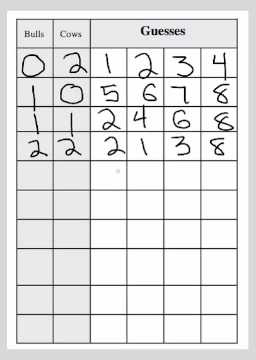
\includegraphics[width=1.0\linewidth,height=0.5\linewidth]{fig080001.png}
   \caption{"Bulls and cows" \\ https://i.ytimg.com/vi/r\_dw8iV\_52g/hqdefault.jpg}
\label{fig080001}
\end{figure}

The Bulls and Cows game (Fig. \ref{fig080001}) is from the group of cipher games. It is played by two players, with paper and pencil, with each player thinking of a four-digit number (secret) that cannot start with the number zero. Each of the players tries to guess the opponent's number. The guessing process involves mentioning a four-digit number, with the opponent responding with information about how many digits of the guess are in their correct places and how many digits are in other places. For each digit that matches in position with the secret number, a bull is reported, and for each digit that does not match in position, a cow is reported. The game ends when one of the players succeeds in guessing a number that results in four bulls.

\section{Designing the GUI}

The game isn't complicated, but it's an ideal way to demonstrate a computer opponent who uses set theory tricks. Game development begins with the creation of a new project (Fig. \ref{fig080002}).

\begin{figure}[H]
   \centering
   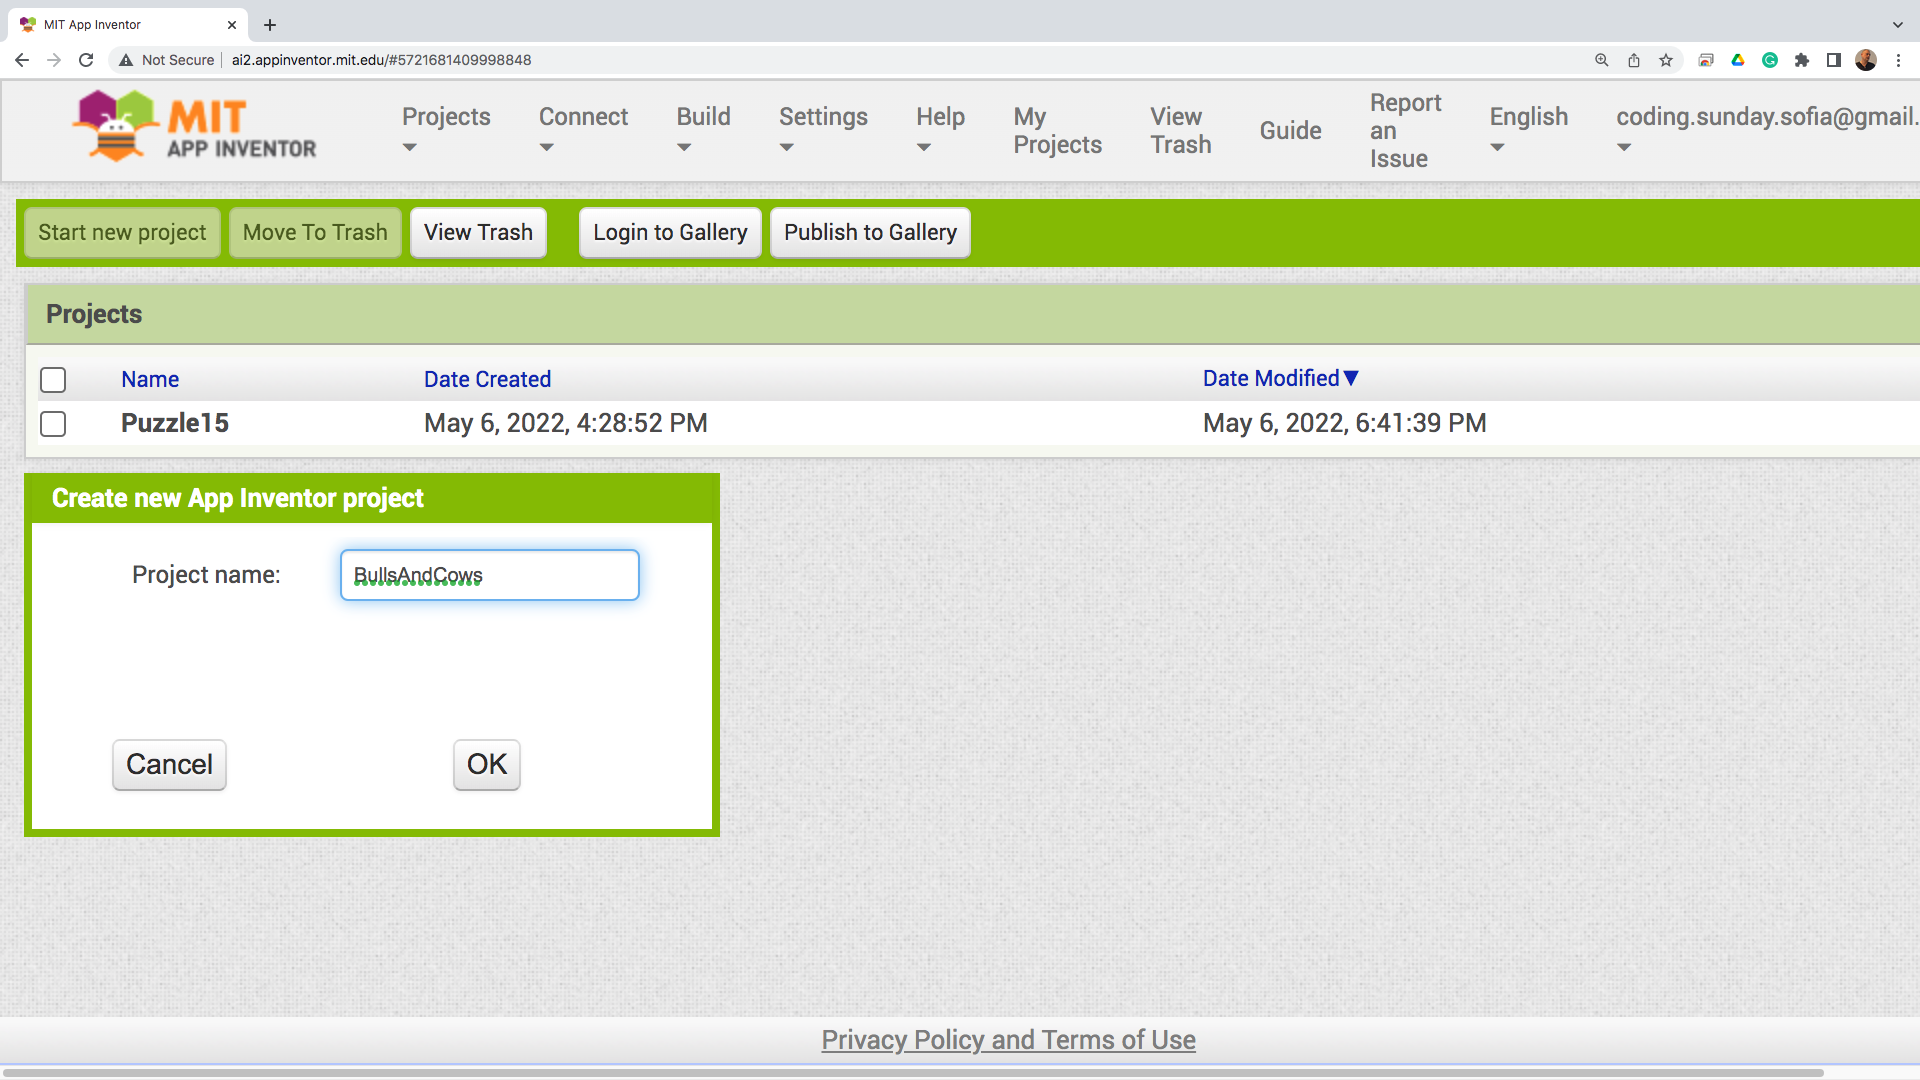
\includegraphics[width=1.0\linewidth,height=0.5\linewidth]{fig080002.png}
   \caption{Creating a new Bulls and Cows project}
\label{fig080002}
\end{figure}

Various ways of organizing the graphical user interface are possible, but for demonstration purposes it is appropriate to use the simplest option. In a table-type visual column control manager, visual controls can be arranged in a matrix of 9 columns and 2 rows (Fig. \ref{fig080003}).

\begin{figure}[H]
   \centering
   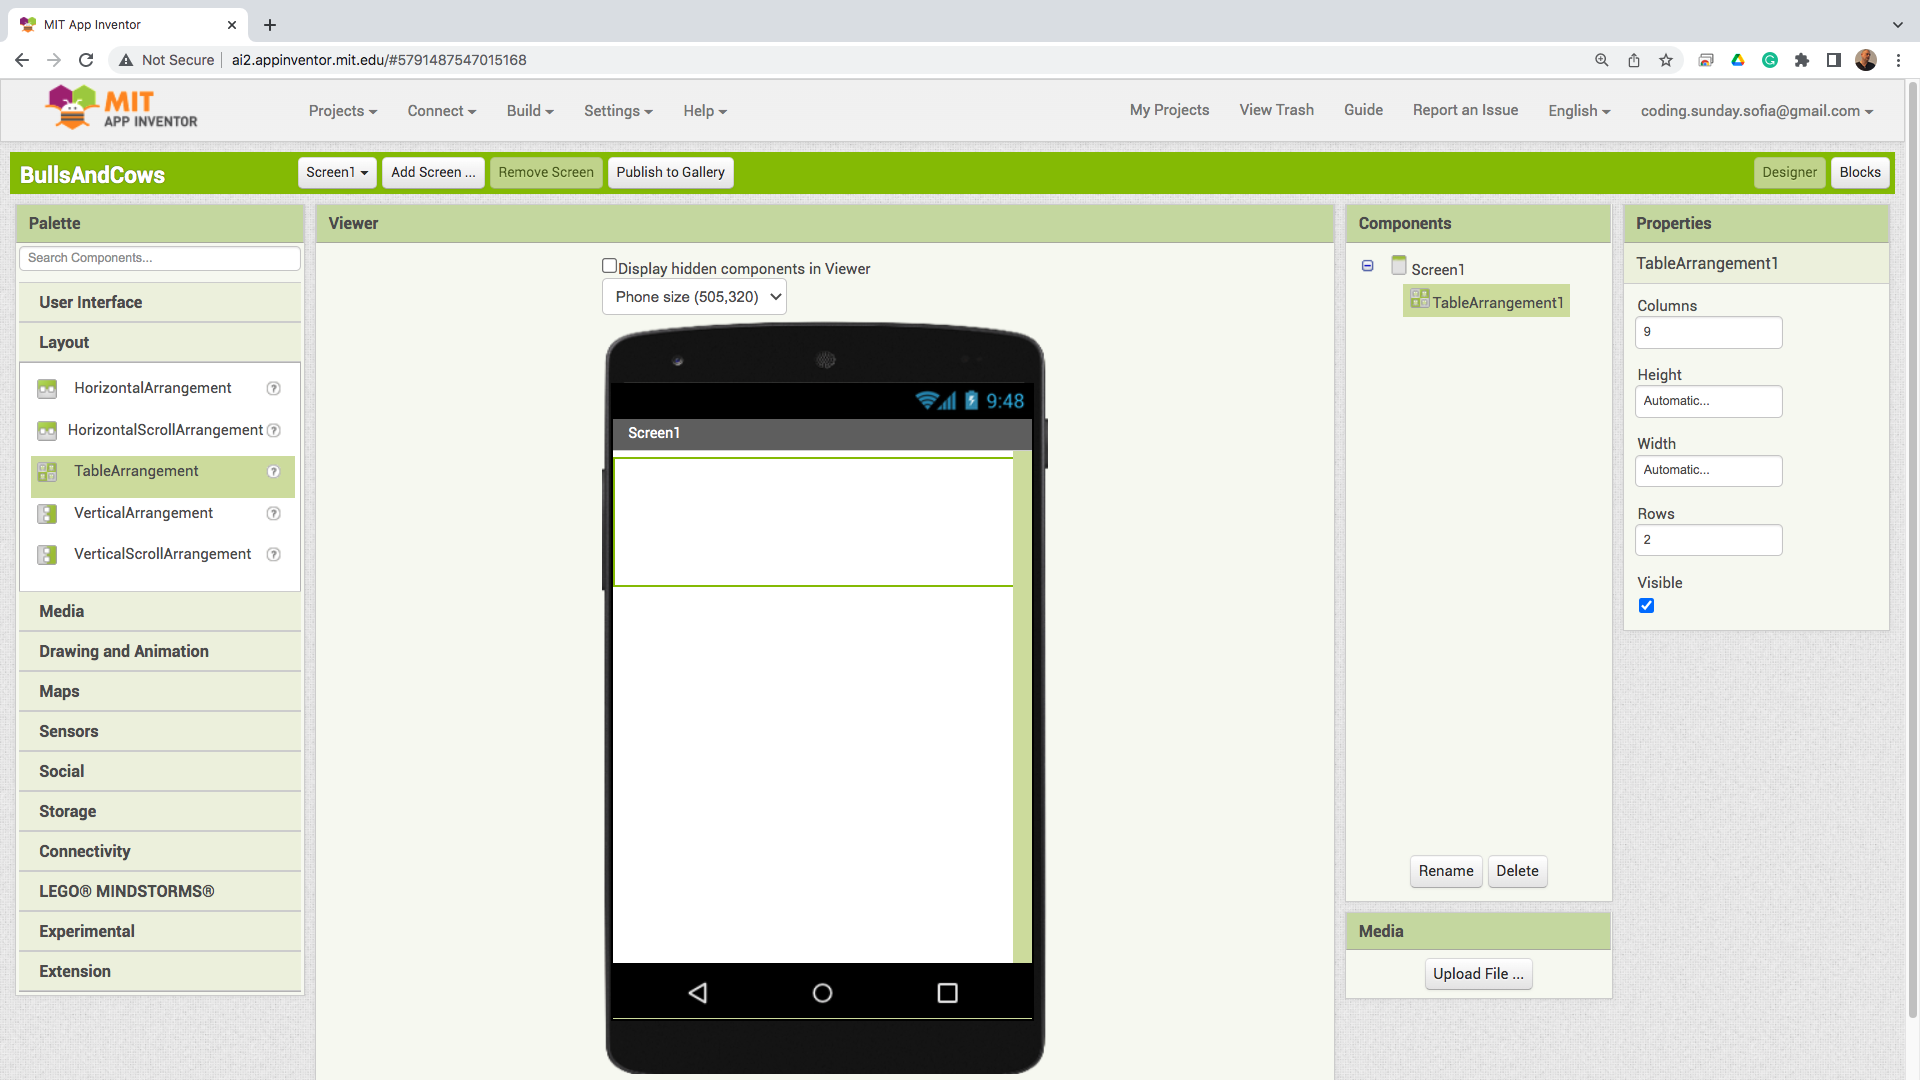
\includegraphics[width=1.0\linewidth,height=0.5\linewidth]{fig080003.png}
   \caption{9x2 Visual Component Manager}
\label{fig080003}
\end{figure}

Since each player queries four digit numbers, the first row in the table, the first four positions, is filled with four visual components to select from a list (Fig. \ref{fig080004}). These four list controls will serve to visualize the four digit numbers guessed by the computer opponent. Each of the components initially displays the star symbol, and the list of possible values is the digits zero through nine. In the first visual component it should not be possible to select the zero, but for symmetry the zero is left in the list.

\begin{figure}[H]
   \centering
   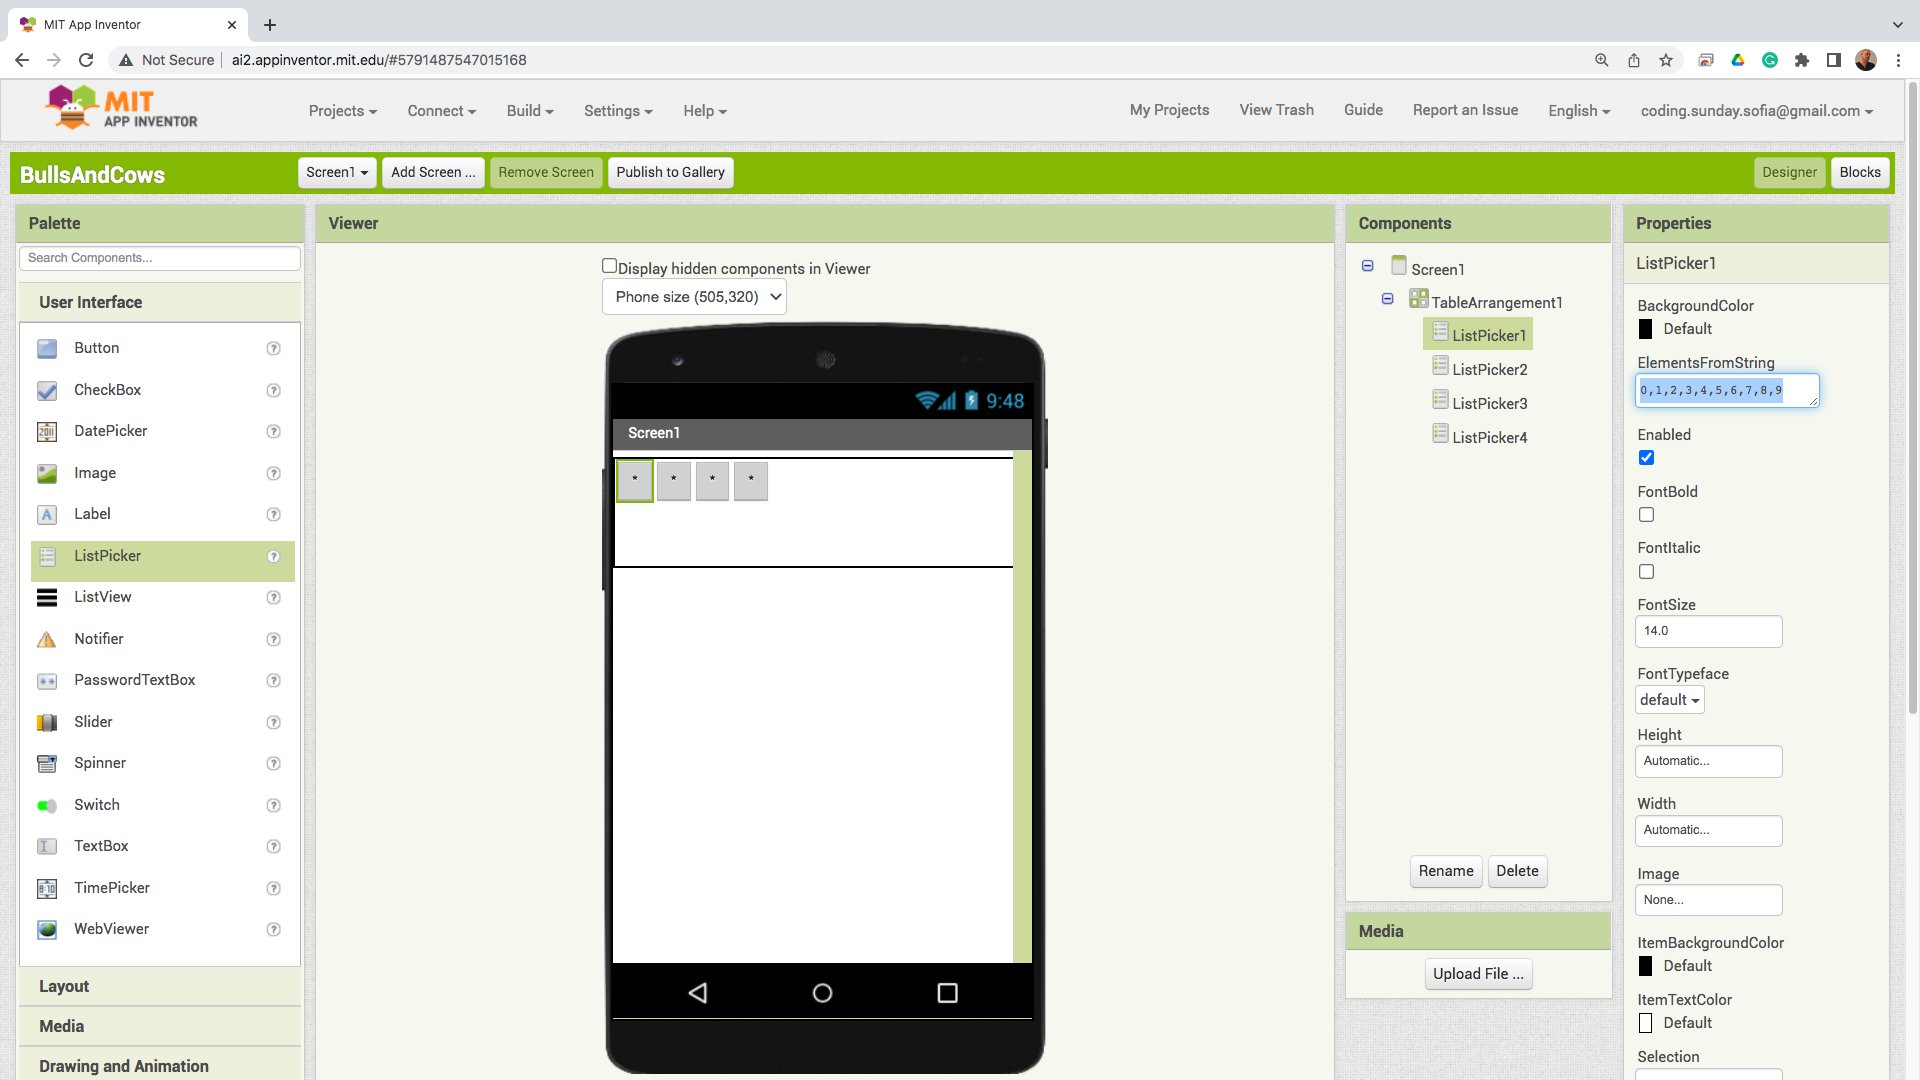
\includegraphics[width=1.0\linewidth,height=0.5\linewidth]{fig080004.png}
   \caption{Visual controls for computer assumptions}
\label{fig080004}
\end{figure}

Similarly, four more list controls (Fig. \ref{fig080005}) are arranged, which will be used by the player to guess what the computer opponent's secret number is. A blank cell is left between the two sets of controls, which will be used for a button to start the guessing procedures.

\begin{figure}[H]
   \centering
   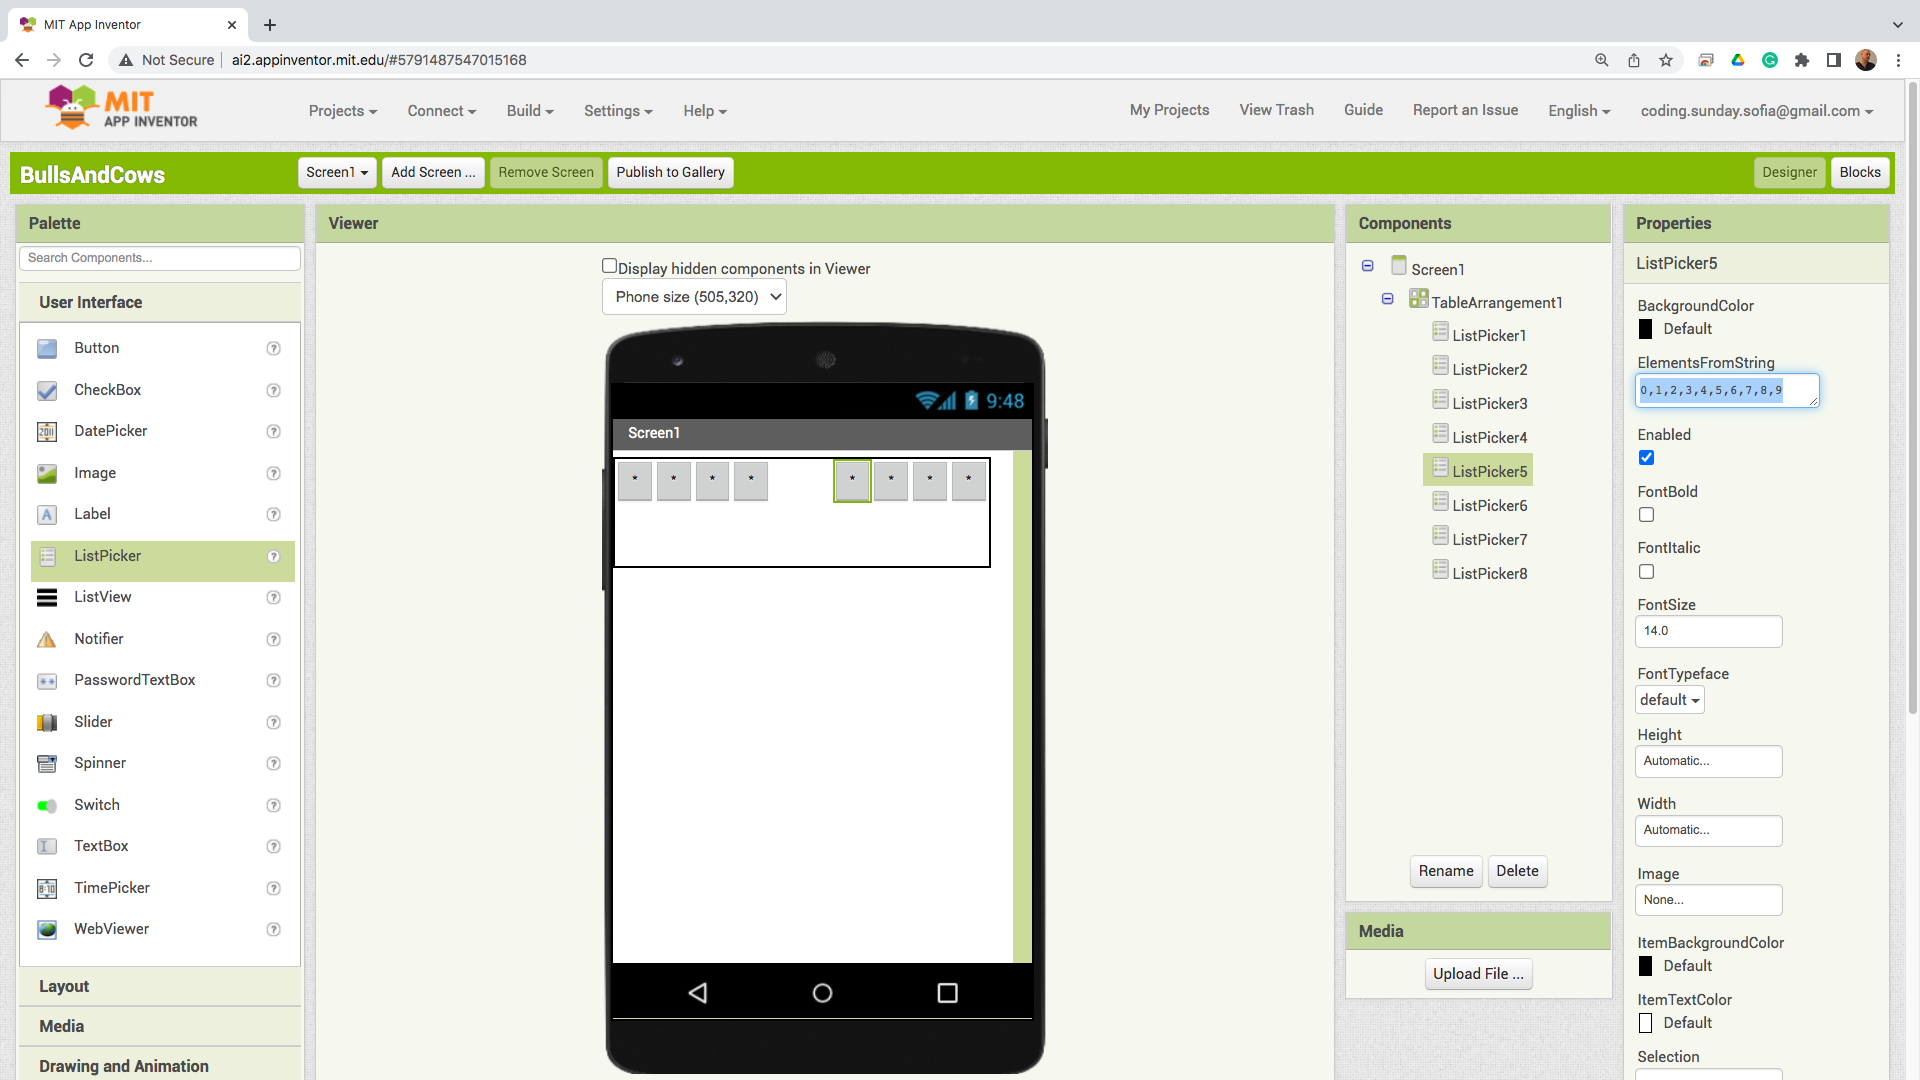
\includegraphics[width=1.0\linewidth,height=0.5\linewidth]{fig080005.png}
   \caption{Visual controls for human assumptions}
\label{fig080005}
\end{figure}

On the second row there are four more list controls that will serve to mark the number of bulls and the number of cows (Fig. \ref{fig080006}). The first two are for the number of bulls and cows known by the computer opponent, and the second two are for the number of bulls and cows known by the player. In pairs, the left control will show the bulls and the right control the cows. The possible options are from zero to four, as the possible bulls or cows are from zero to four inclusive.

\begin{figure}[H]
   \centering
   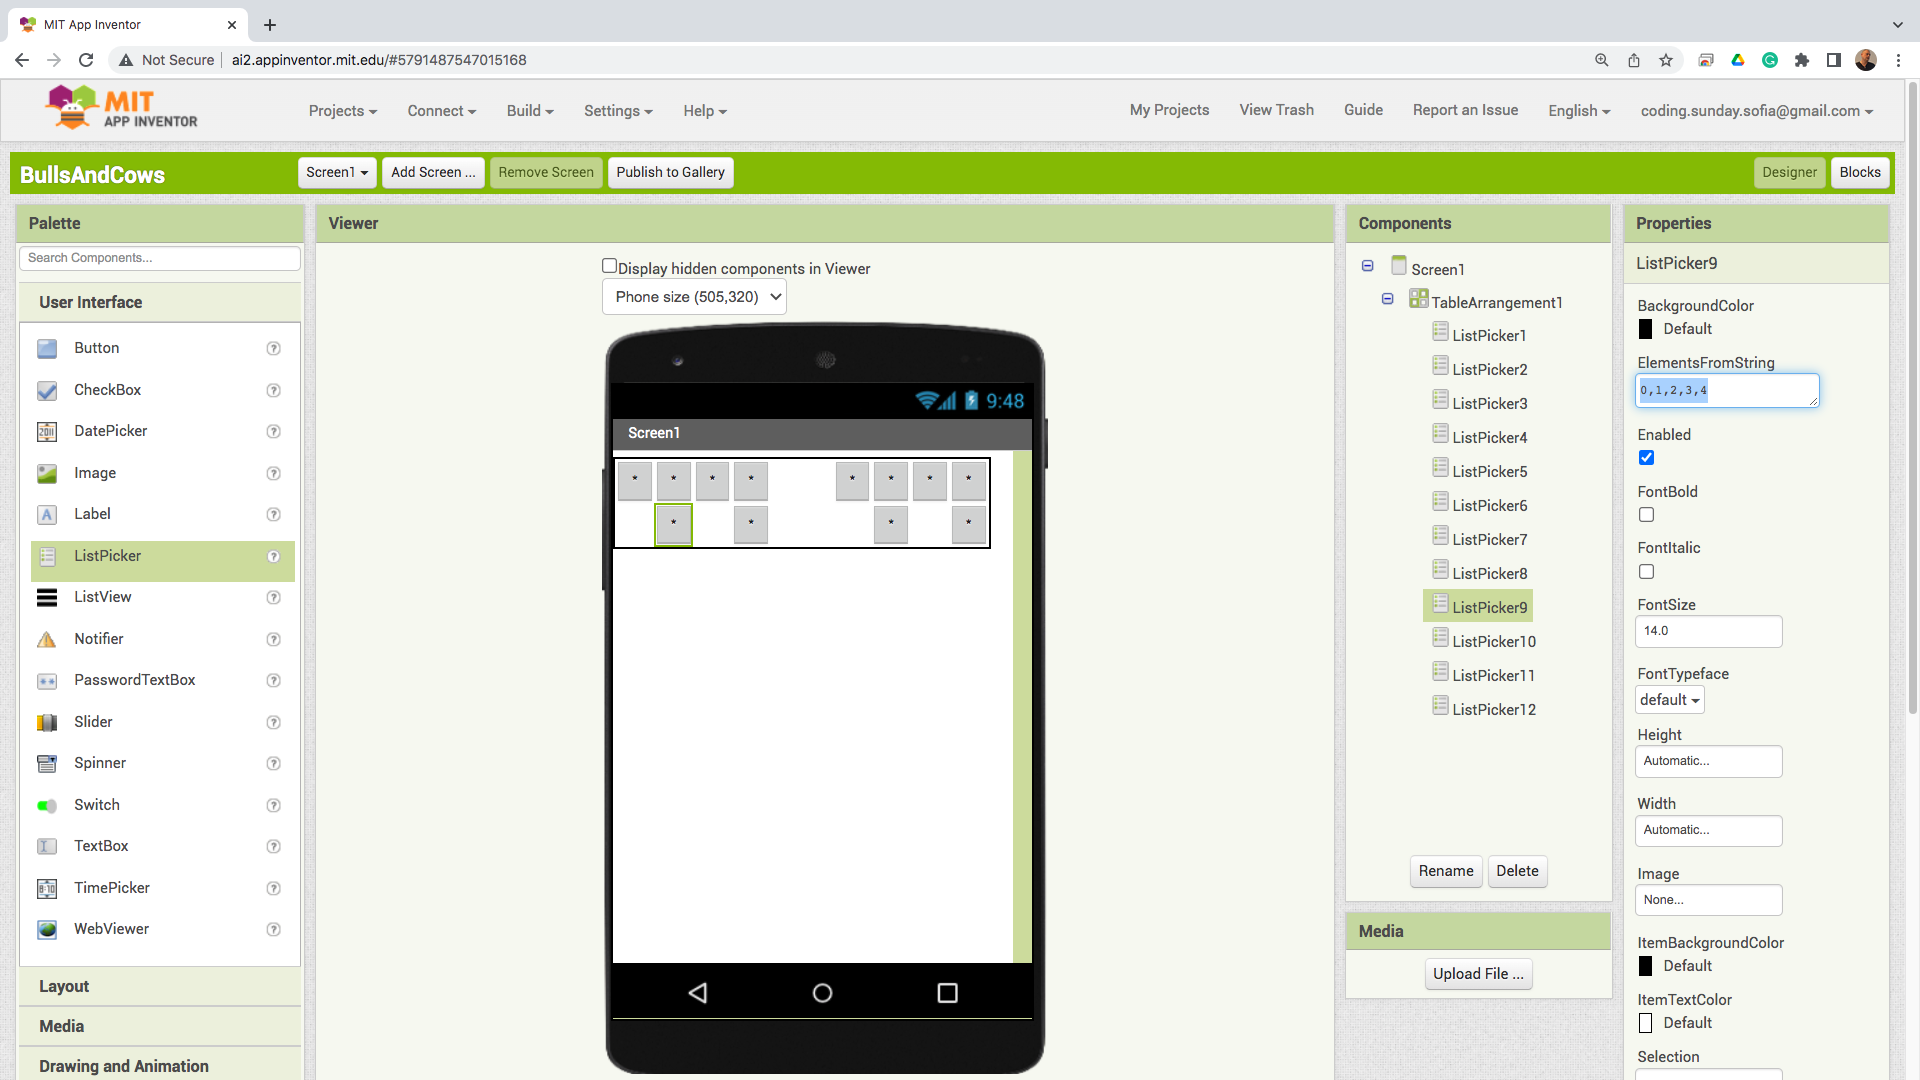
\includegraphics[width=1.0\linewidth,height=0.5\linewidth]{fig080006.png}
   \caption{Visual controls for counting bulls and cows}
\label{fig080006}
\end{figure}

List selection components do not display the selected option in their text automatically. For this reason, it is necessary to intercept the selection made event and write the selected option to the text field of the visual component. For this purpose, a common event generated by all list components on the screen is caught (Fig. \ref{fig080007}).

\begin{figure}[H]
   \centering
   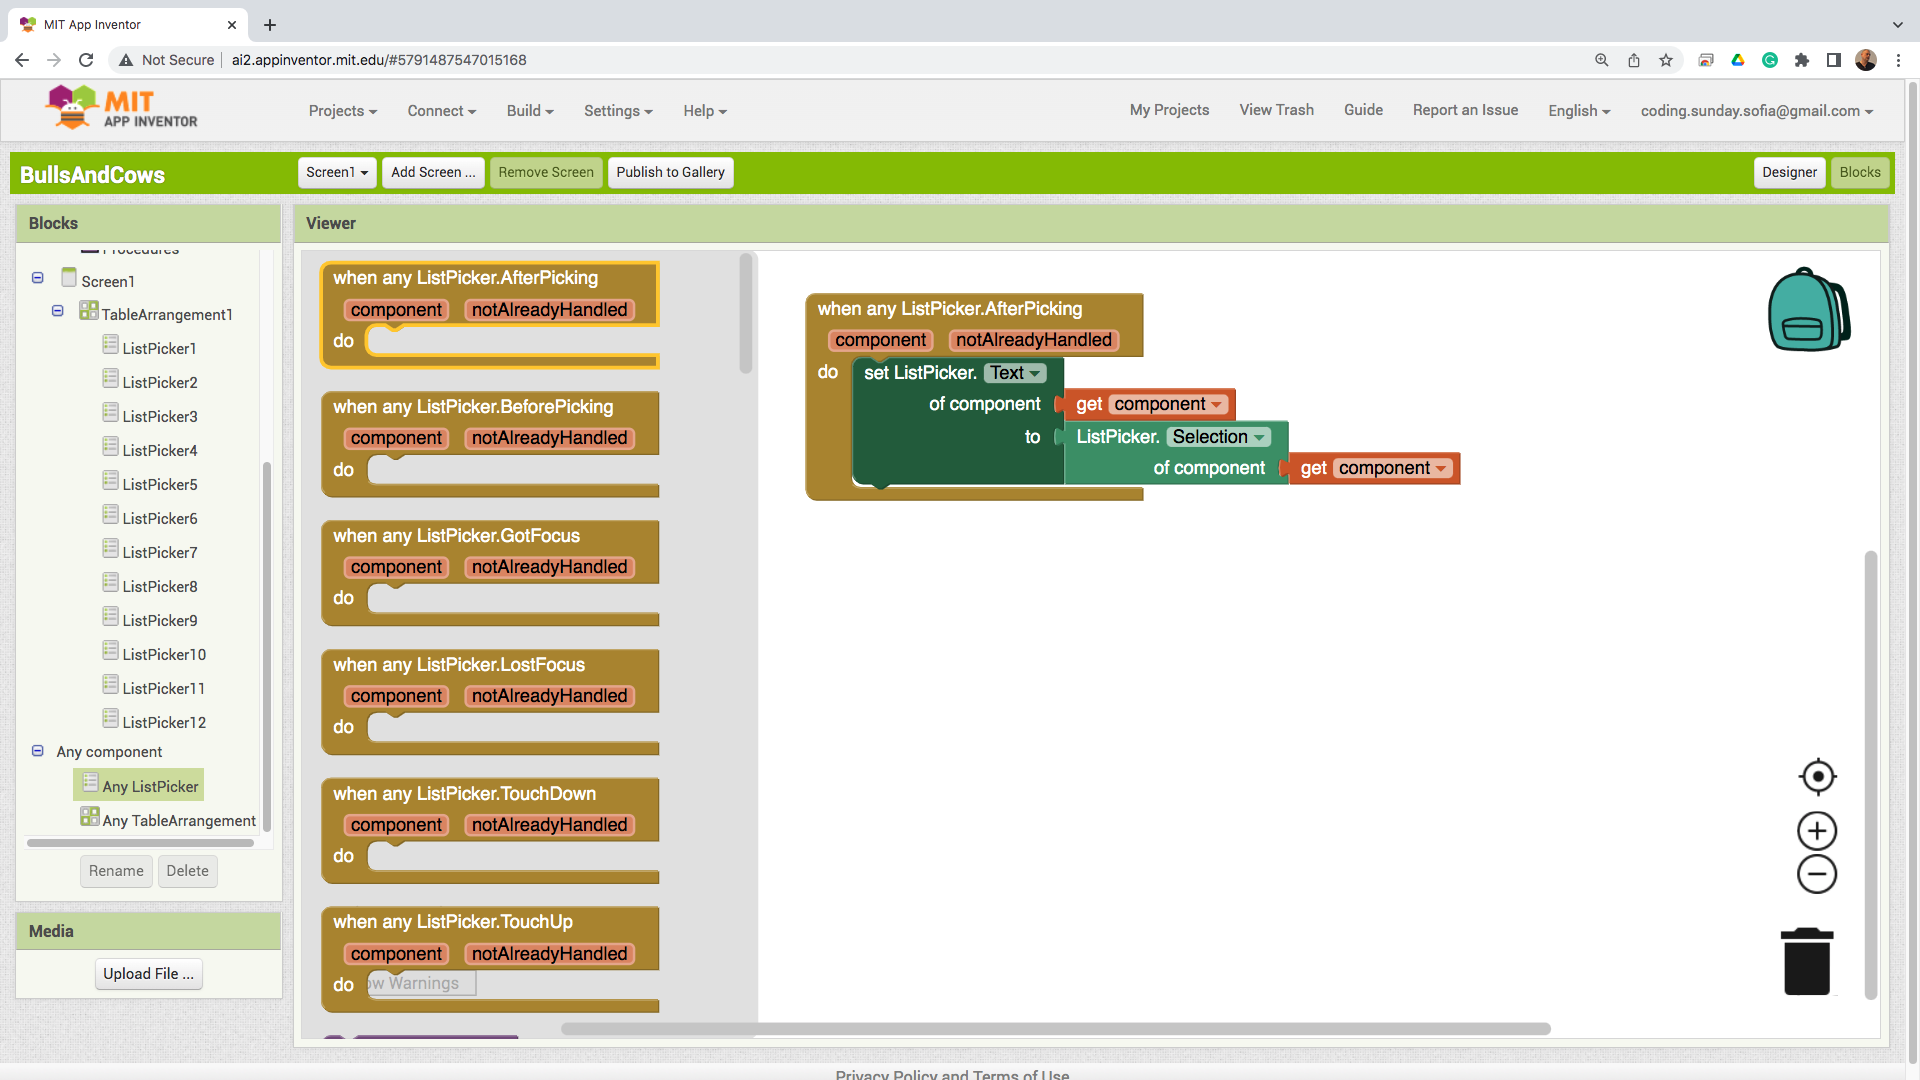
\includegraphics[width=1.0\linewidth,height=0.5\linewidth]{fig080007.png}
   \caption{Preview of selected option}
\label{fig080007}
\end{figure}

It is reasonable to place labels in front of the cells for counting the number of bulls and the number of cows (Fig. \ref{fig080008}). The Latin letter B is used for the bulls and the Latin letter C for the number of cows.

\begin{figure}[H]
   \centering
   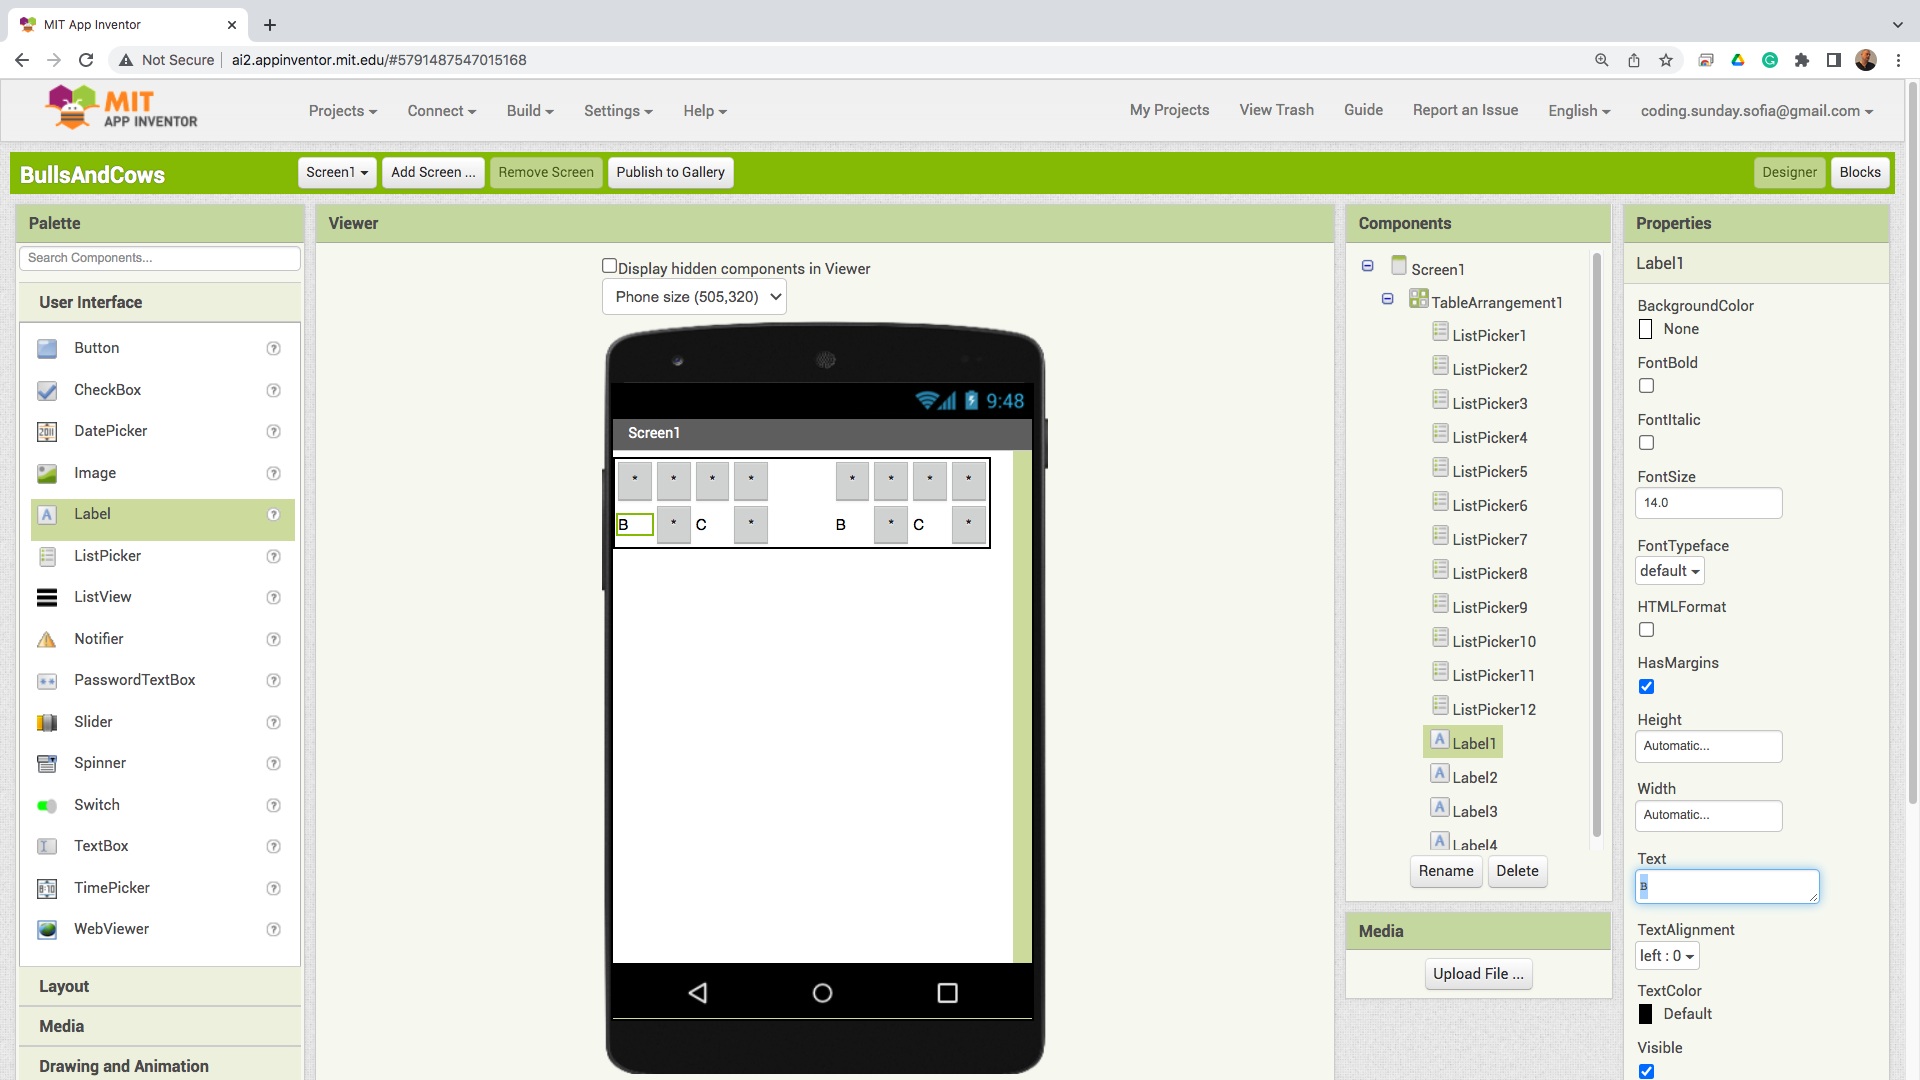
\includegraphics[width=1.0\linewidth,height=0.5\linewidth]{fig080008.png}
   \caption{Labels in front of bull and cow counting controls}
\label{fig080008}
\end{figure}

The user interface ends with two buttons (Fig. \ref{fig080009}). The first activates the computer opponent to guess the player's number, and the second prompts the computer opponent to report the number of bulls and cows hit by the human.

\begin{figure}[H]
   \centering
   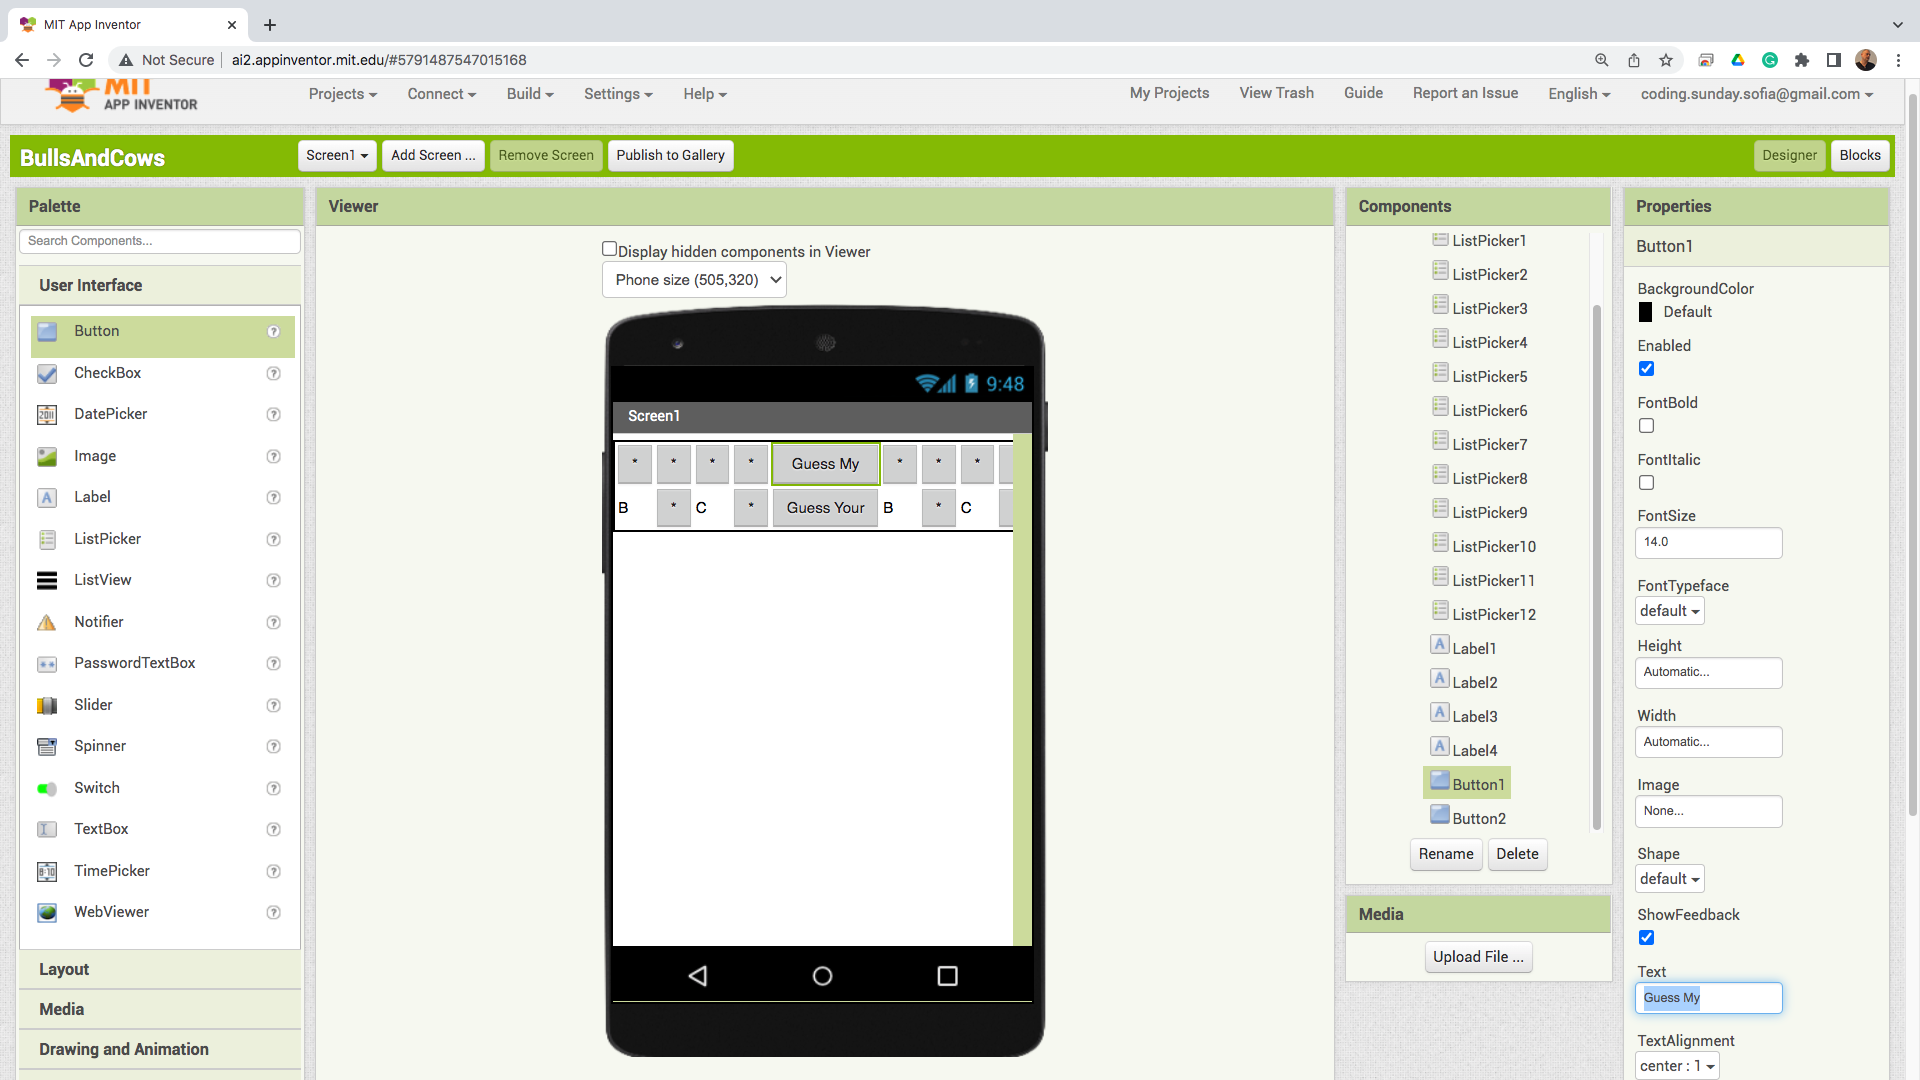
\includegraphics[width=1.0\linewidth,height=0.5\linewidth]{fig080009.png}
   \caption{Buttons to activate the guessing process}
\label{fig080009}
\end{figure}

\section{Using Data Structures}

For the needs of the computer adversary and according to set theory, it is important to create a list structure (Fig. \ref{fig080010}) that contains all possible combinations of four-digit numbers, the digits of which do not repeat and do not start with zero . For each person's response, all combinations that do not meet the conditions for established bulls and cows are excluded from the list.

\begin{figure}[H]
   \centering
   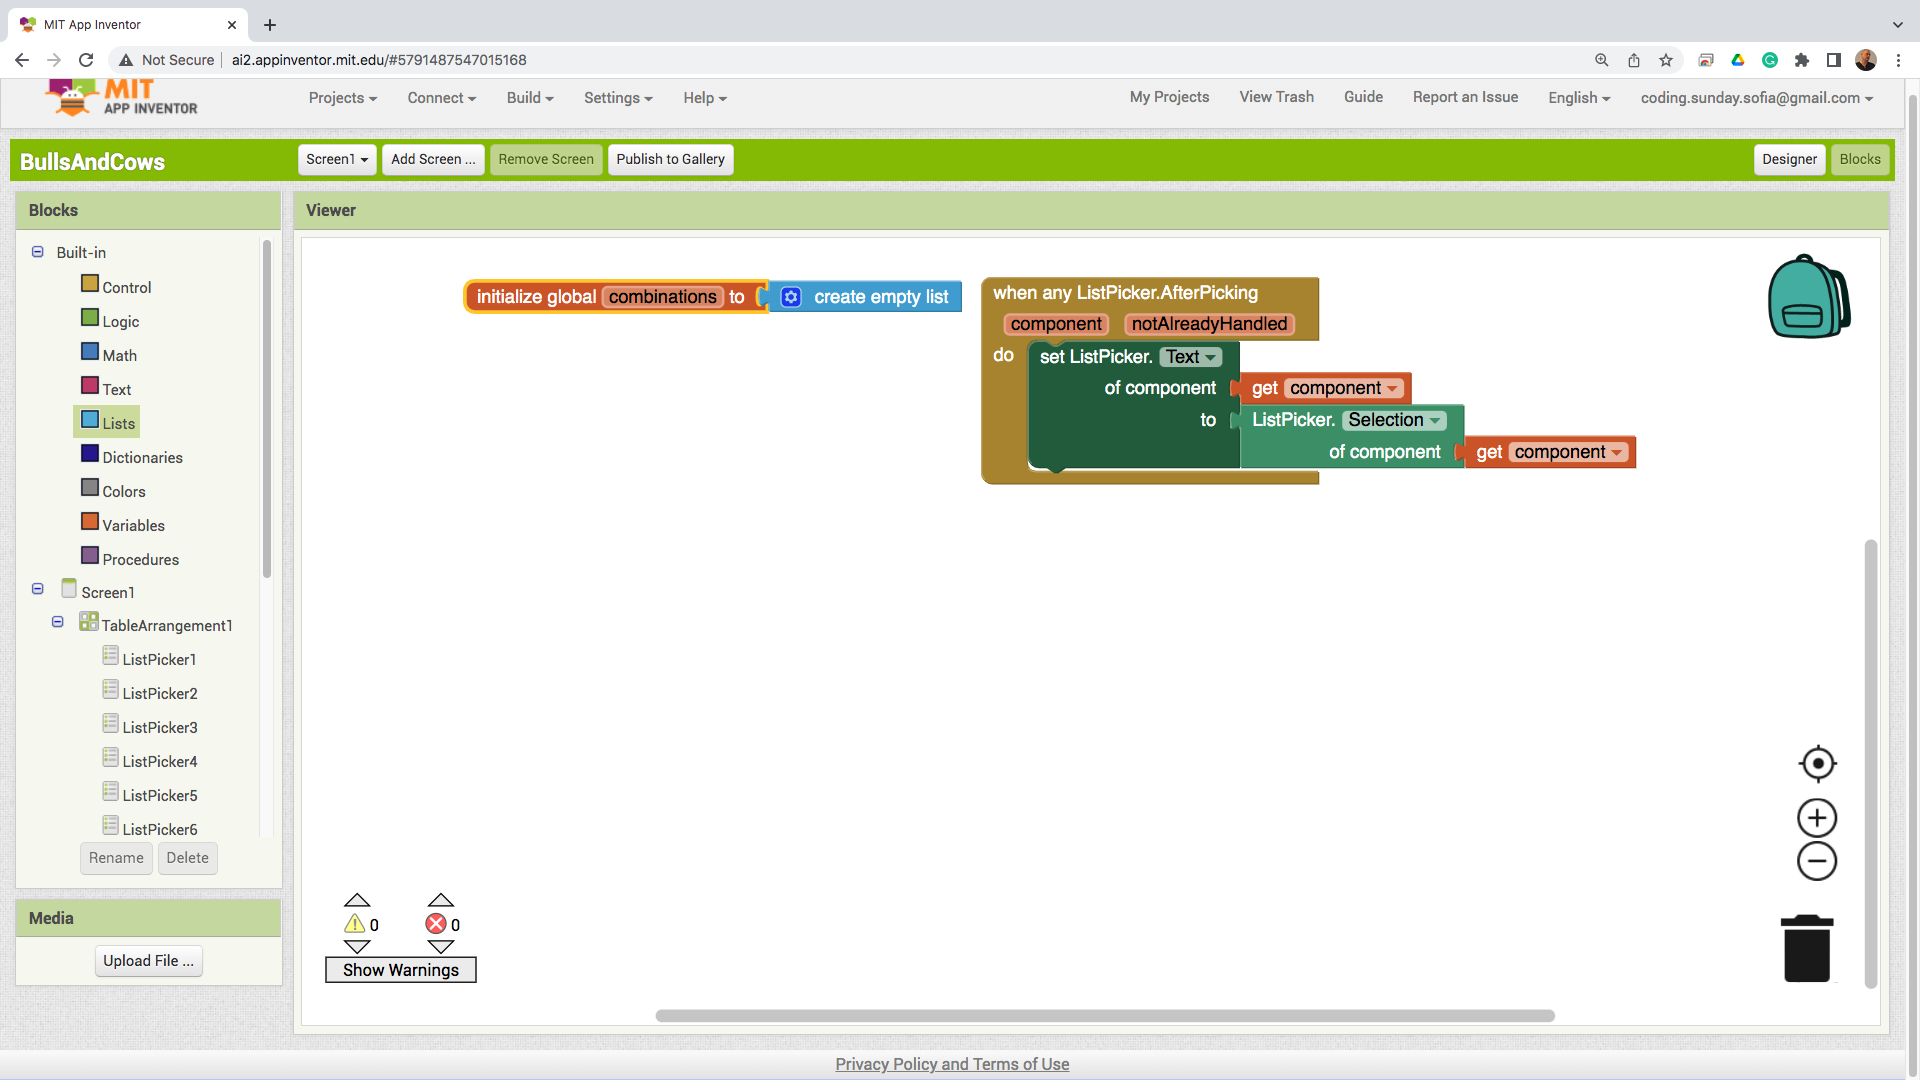
\includegraphics[width=1.0\linewidth,height=0.5\linewidth]{fig080010.png}
   \caption{List of combinations}
\label{fig080010}
\end{figure}

The numbers are four digits, so the list of combinations can be filled using four loops (Fig. \ref{fig080011}). The first rotates from one to nine, since zero cannot participate as the first digit. The other three cycles rotate from zero to nine. The Latin letters a, b, c and d are chosen as cycle counters. Each of the counters will participate in the formation of a four-digit number.

\begin{figure}[H]
   \centering
   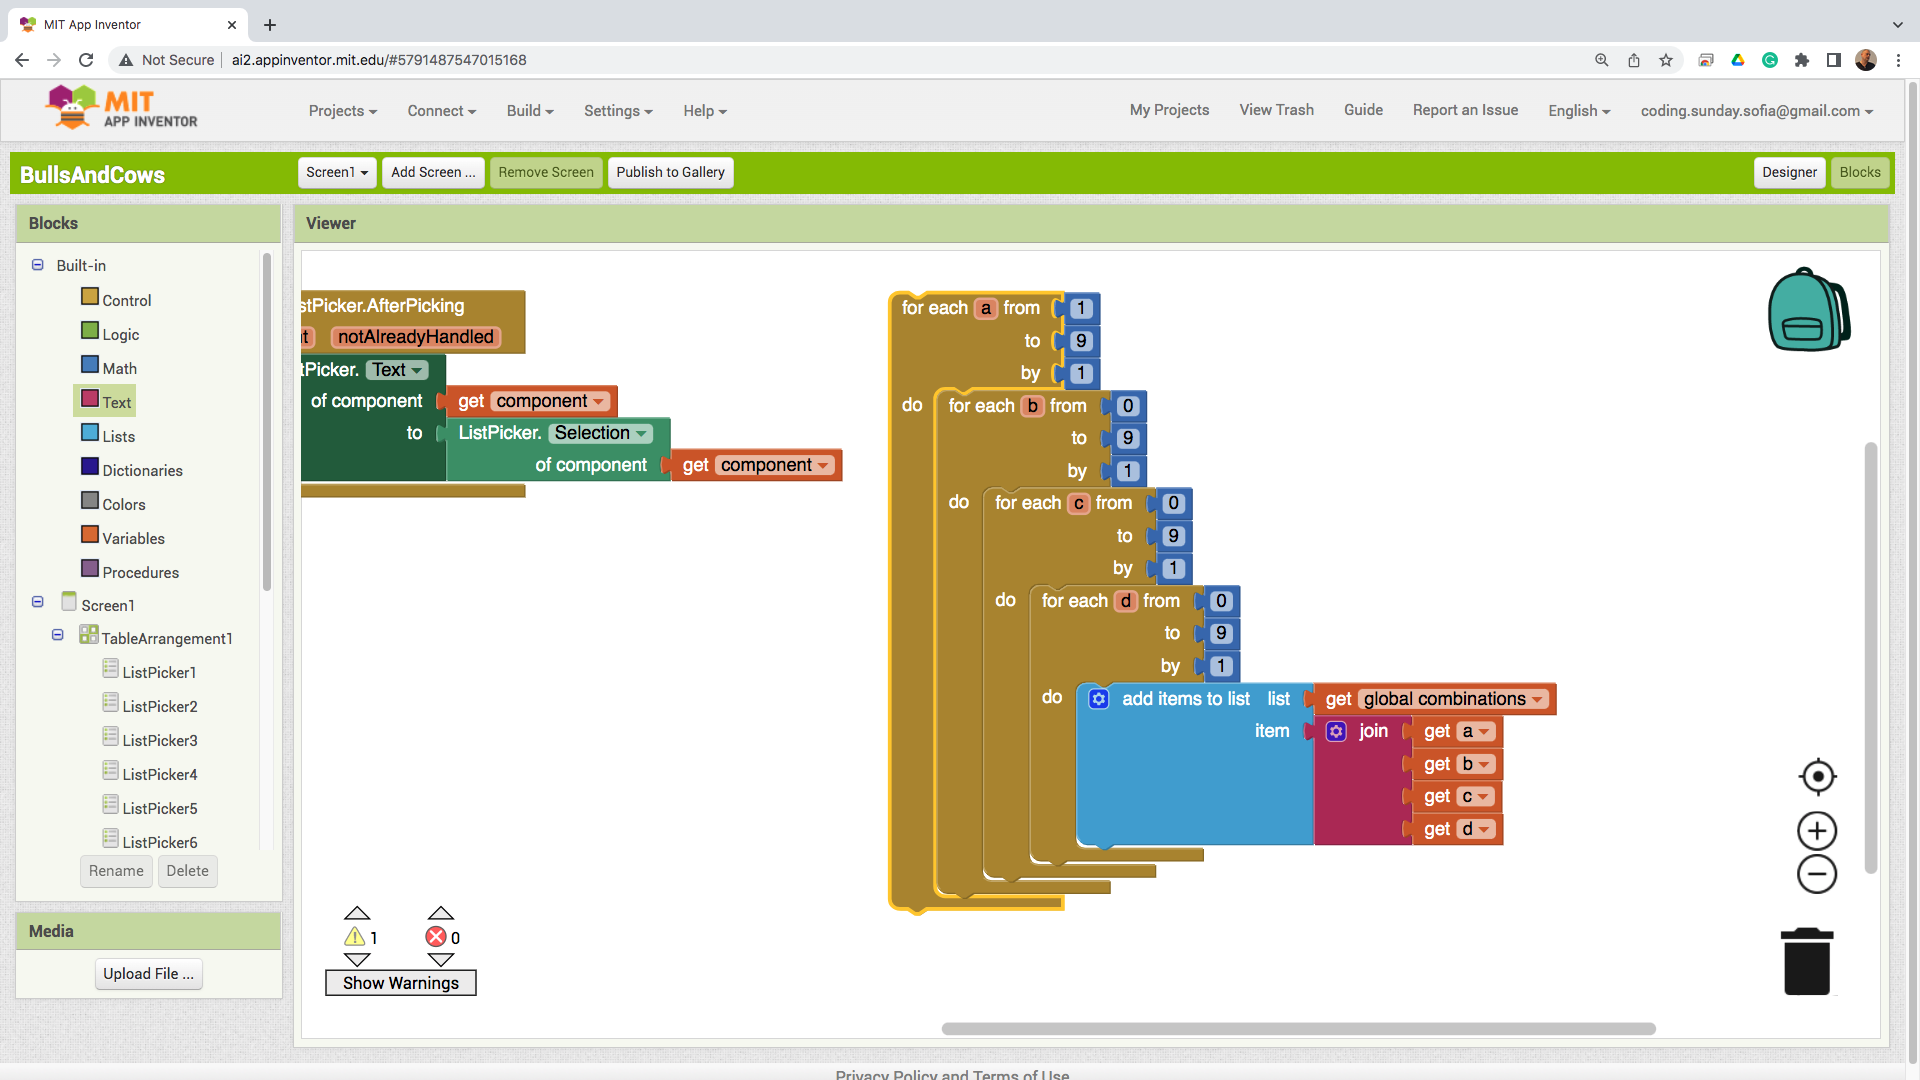
\includegraphics[width=1.0\linewidth,height=0.5\linewidth]{fig080011.png}
   \caption{Cycles to generate the combinations}
\label{fig080011}
\end{figure}

In order to avoid repeating the numbers, a series of checks must be made (Fig. \ref{fig080012}). For the first loop, no check will be made, but the second loop is rotated only if counter b differs from counter a. The third loop is looped only if counter c differs from counter a and counter c differs from counter b. The fourth loop only rotates if counter d is different from counter a, different from counter b, and different from counter c.

\begin{figure}[H]
   \centering
   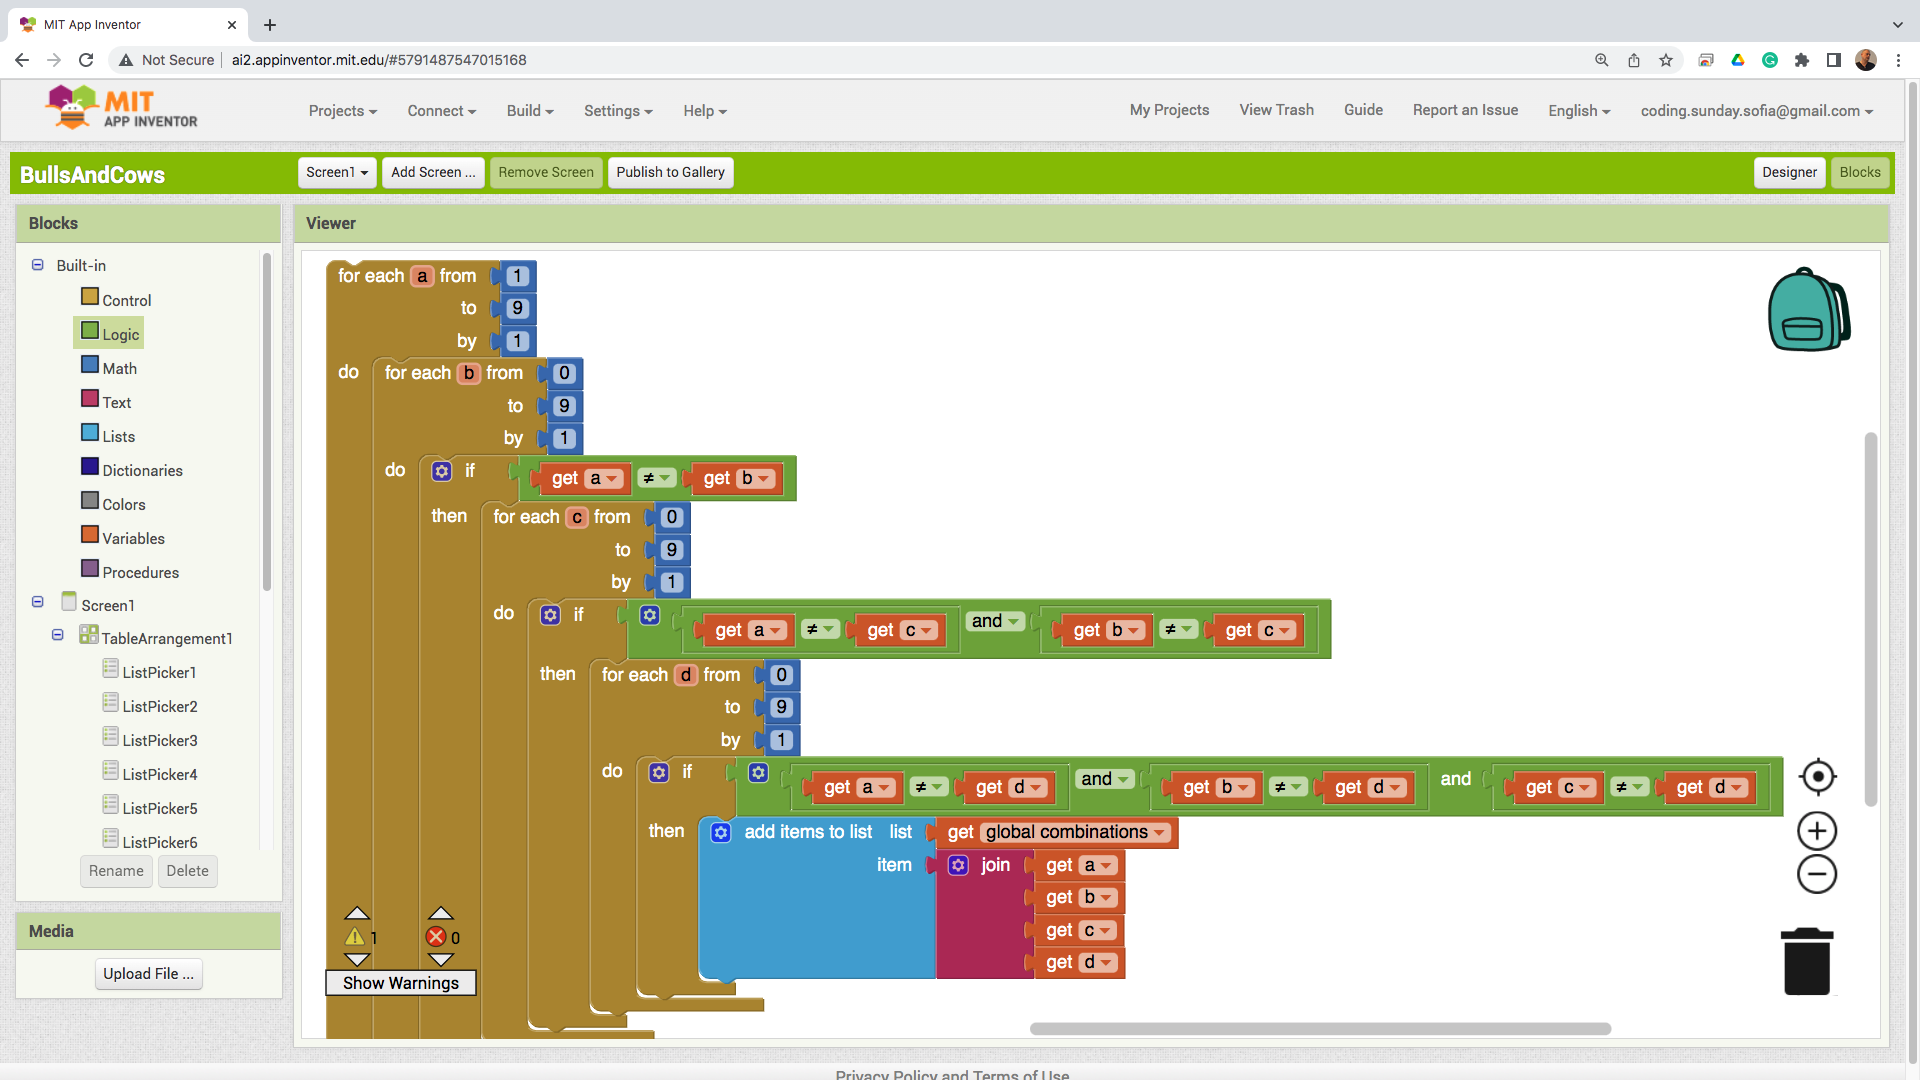
\includegraphics[width=1.0\linewidth,height=0.5\linewidth]{fig080012.png}
   \caption{Checks to avoid duplicate digits}
\label{fig080012}
\end{figure}

Two global variables help store the secret numbers for the computer opponent and the human opponent (Fig. \ref{fig080013}). Two more global variables help handle the computer opponent's guess and the human guess. All four variables are initially initialized to zeros.

\begin{figure}[H]
   \centering
   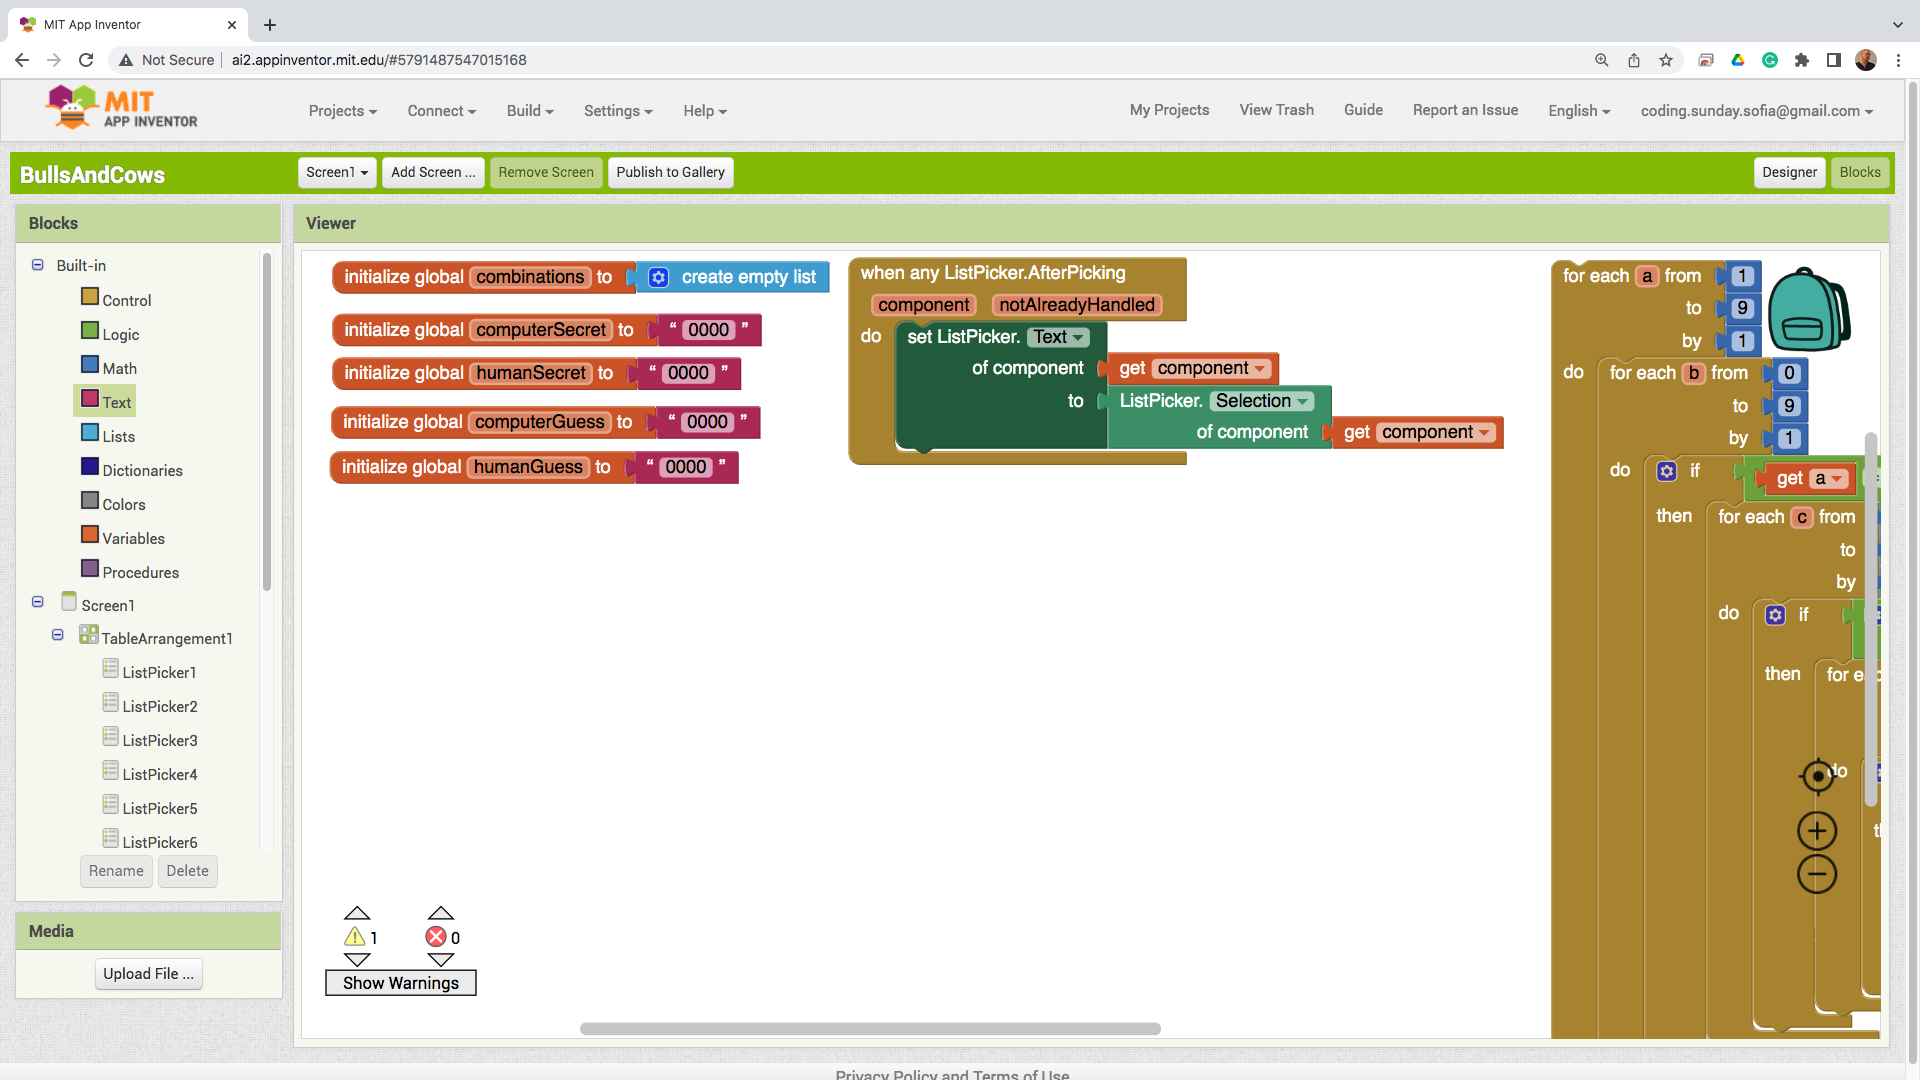
\includegraphics[width=1.0\linewidth,height=0.5\linewidth]{fig080013.png}
   \caption{Helper variables for players' secret numbers}
\label{fig080013}
\end{figure}

\section{Game Manipulation Algorithms}

The cycles for initializing the list of combinations and the subsequent selection of one of them as the computer opponent's secret number must occur in an event marking the initialization of the work screen (Fig. \ref{fig080014}).

\begin{figure}[H]
   \centering
   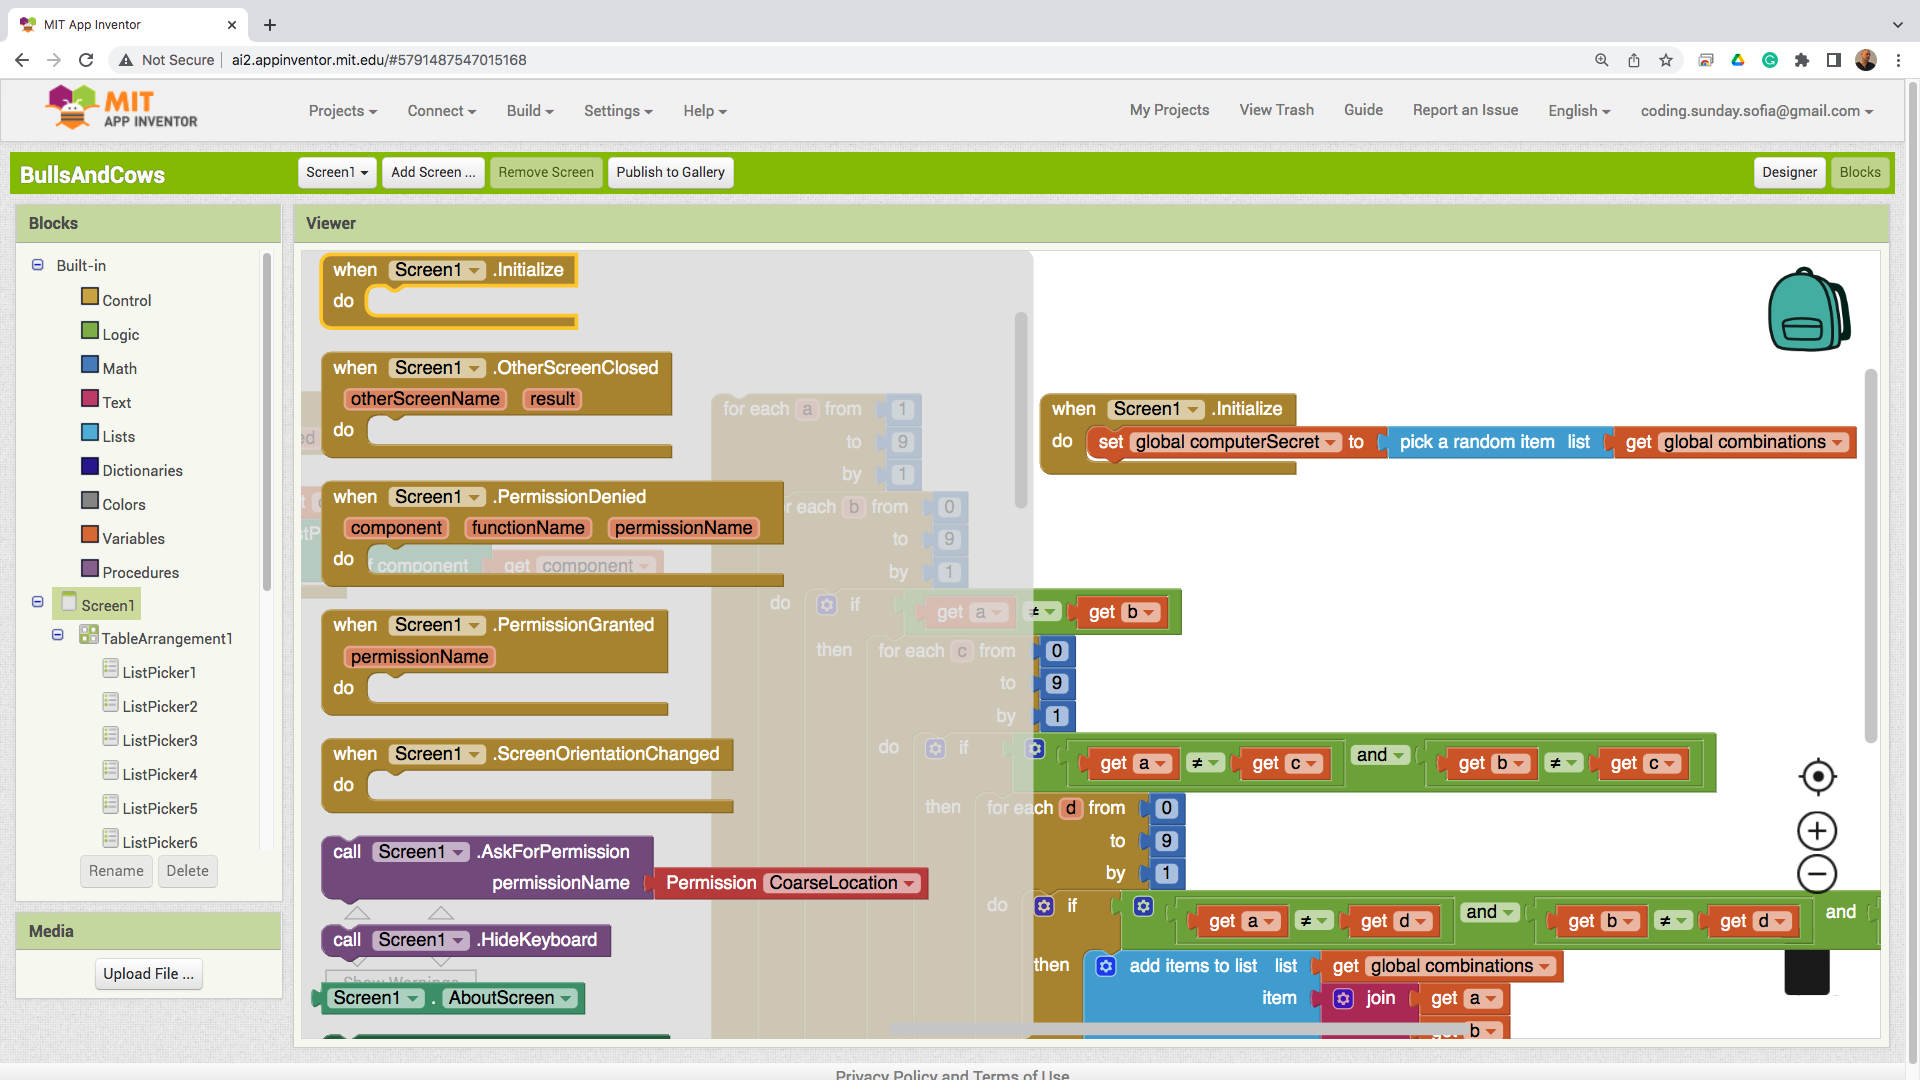
\includegraphics[width=1.0\linewidth,height=0.5\linewidth]{fig080014.png}
   \caption{Initial screen initialization}
\label{fig080014}
\end{figure}

The task of the first button is to take a guess from the computer opponent (calling an additional procedure) and reset all other digits on the visual components (Fig. \ref{fig080015}).

\begin{figure}[H]
   \centering
   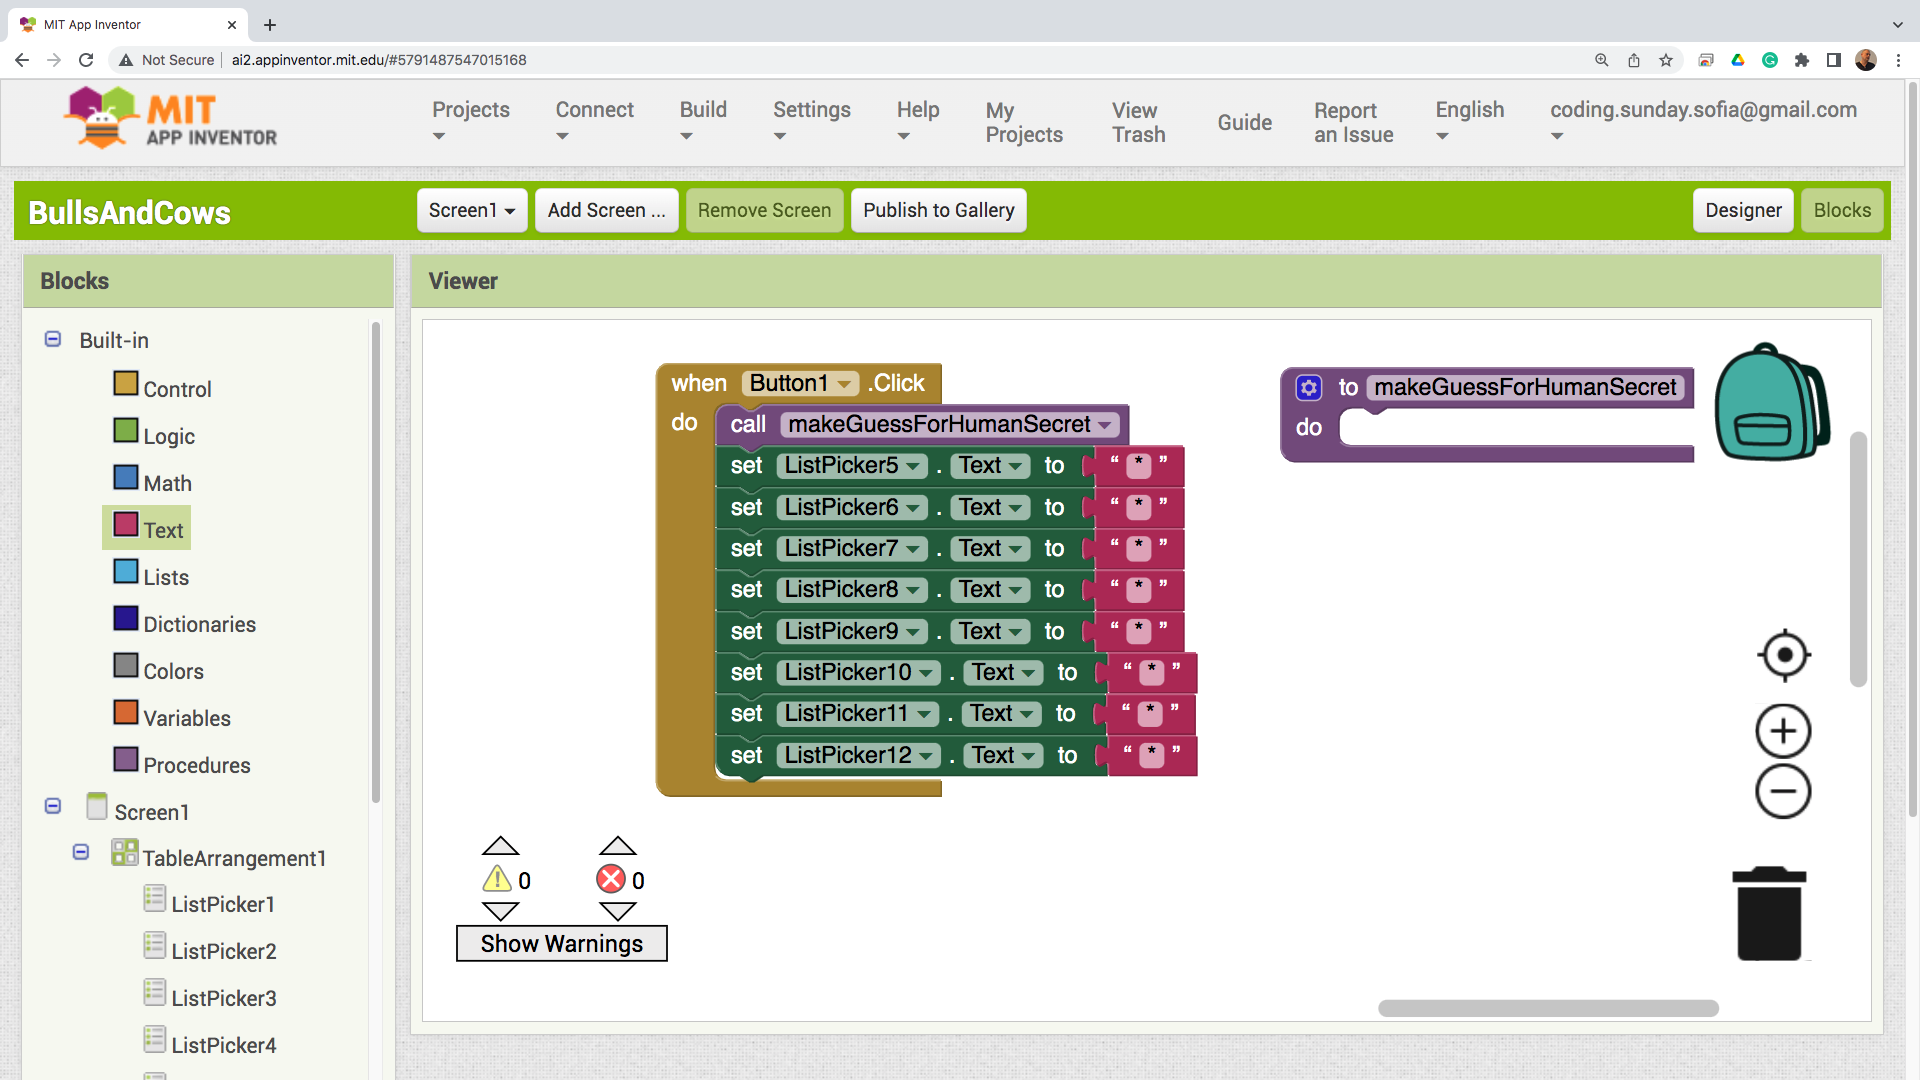
\includegraphics[width=1.0\linewidth,height=0.5\linewidth]{fig080015.png}
   \caption{First Button Actions}
\label{fig080015}
\end{figure}

The computer opponent guesses the player's secret number by choosing one item from the list of remaining combinations. If the list is empty (Fig. \ref{fig080016}), then this means that the person has given incorrect information on one of the previous moves and knowing his number is impossible. In the notification component, a message is issued that the game cannot continue.

\begin{figure}[H]
   \centering
   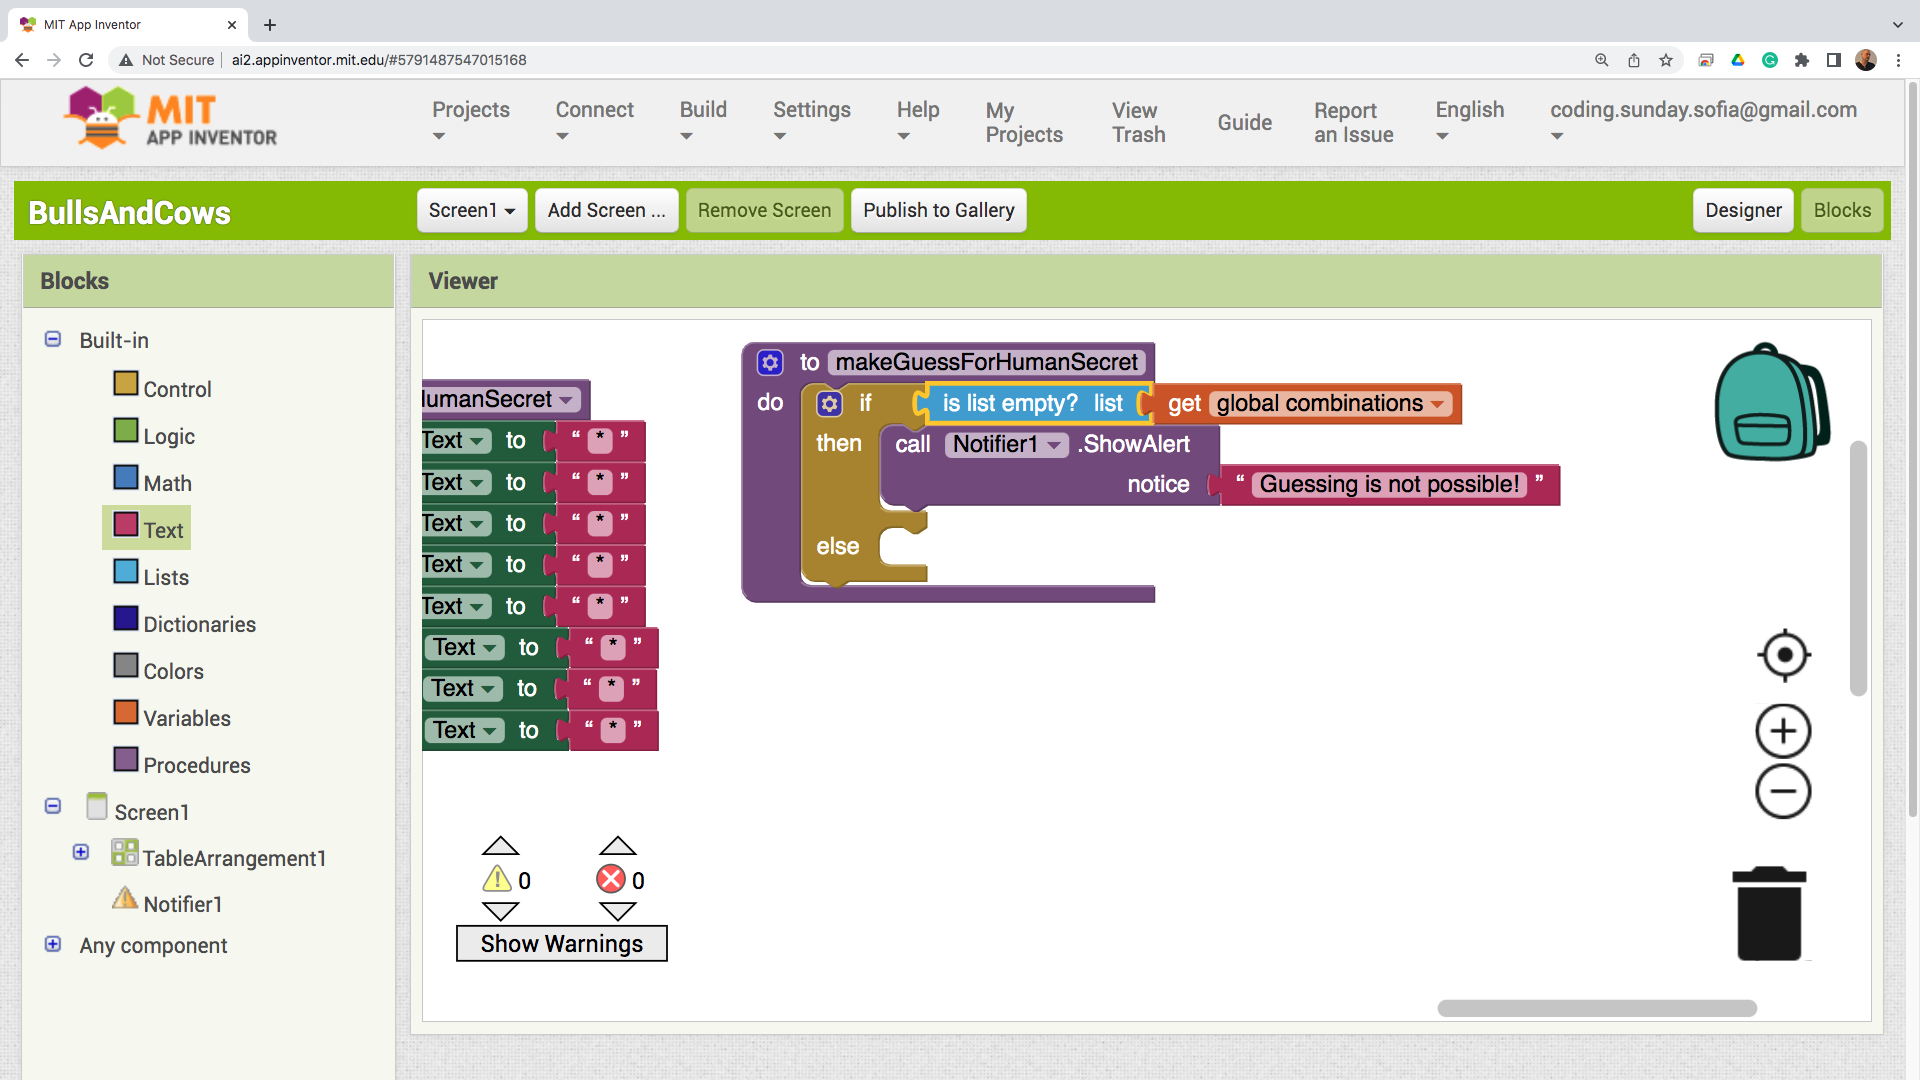
\includegraphics[width=1.0\linewidth,height=0.5\linewidth]{fig080016.png}
   \caption{Checking for remaining available combinations}
\label{fig080016}
\end{figure}

If there are elements in the list of combinations, one of the elements is chosen at random (Fig. \ref{fig080017}). The selected number is visualized in the first four cells of the interface, taking the individual digits for this purpose.

\begin{figure}[H]
   \centering
   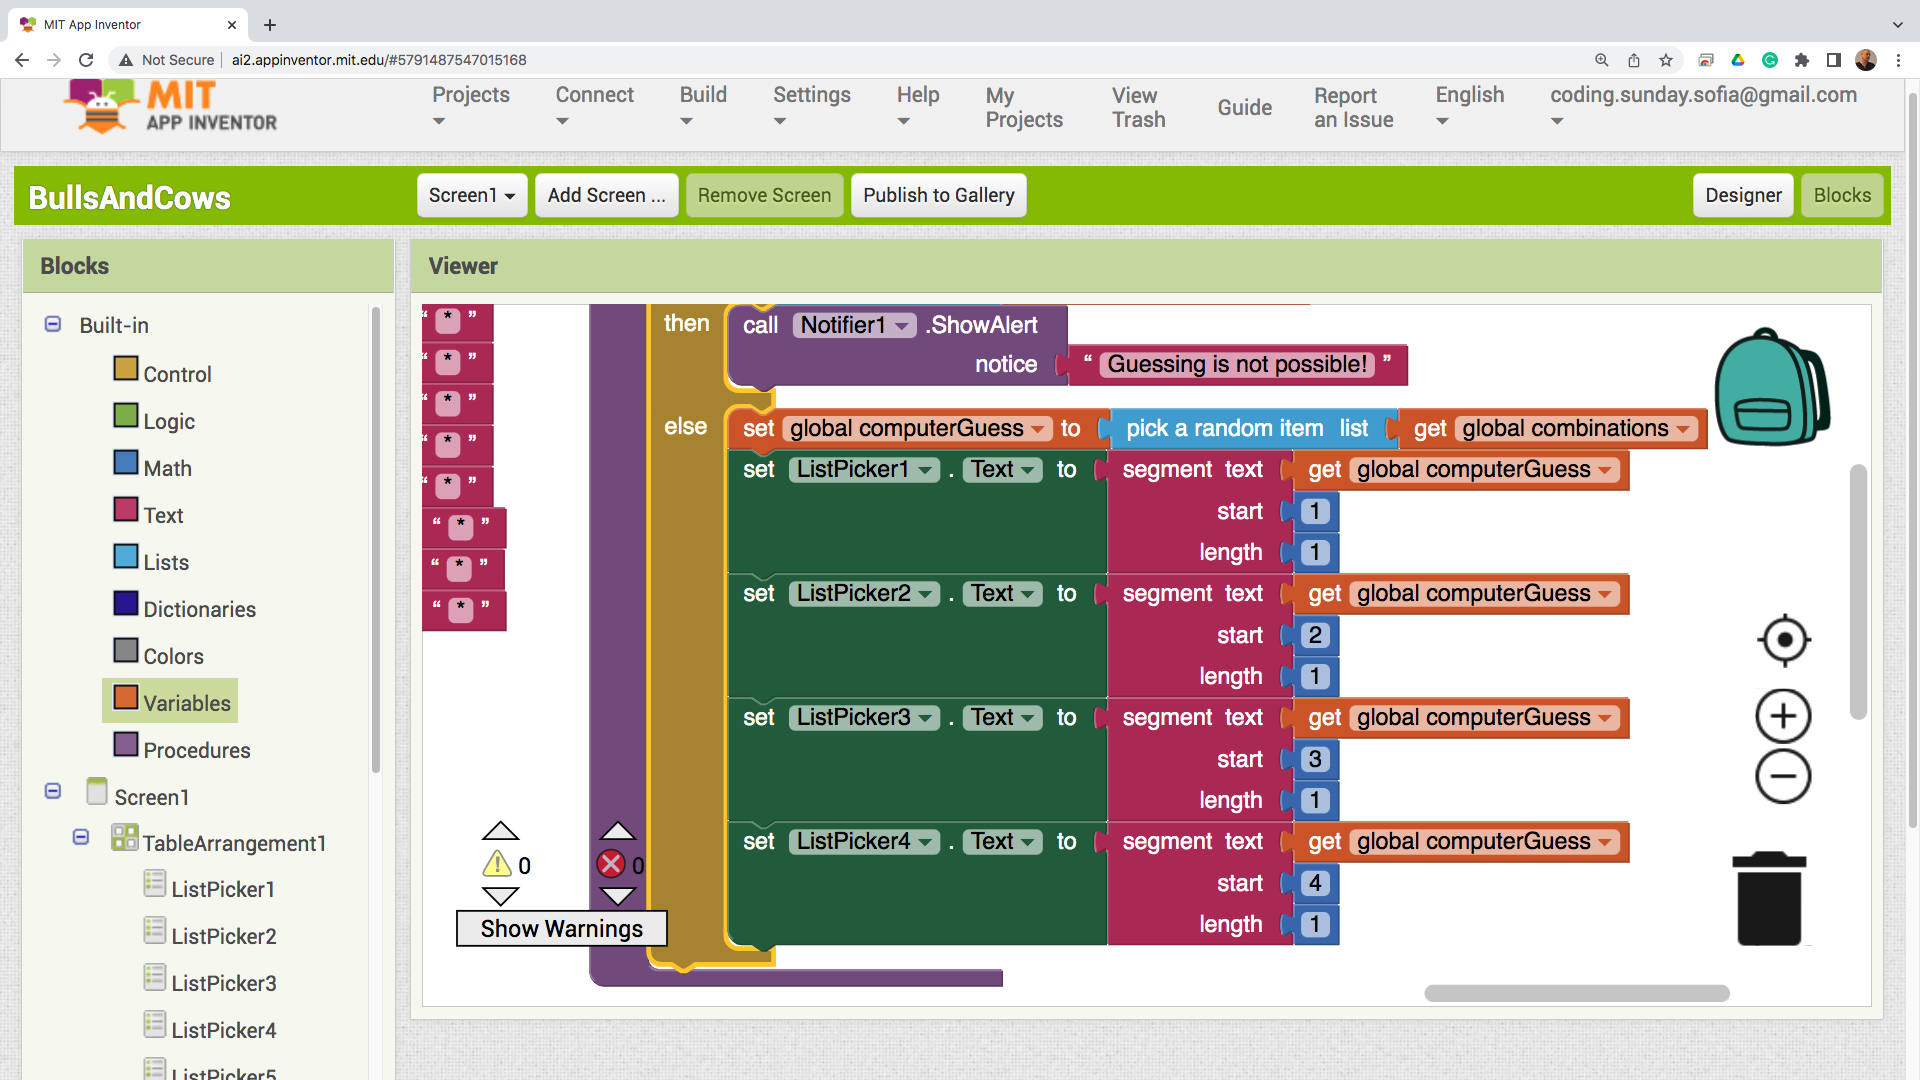
\includegraphics[width=1.0\linewidth,height=0.5\linewidth]{fig080017.png}
   \caption{Choose a number to guess}
\label{fig080017}
\end{figure}

When the second button is pressed, three actions are performed, and for each of them a helper procedure is called (Fig. \ref{fig080018}). First, the information is taken from the visual controls, for the assumption made by the person. The second action is to visualize the number of bulls and cows hit by the human. The third action is to exclude all combinations in the list that do not meet the criteria of the last guess made by the computer opponent.

\begin{figure}[H]
   \centering
   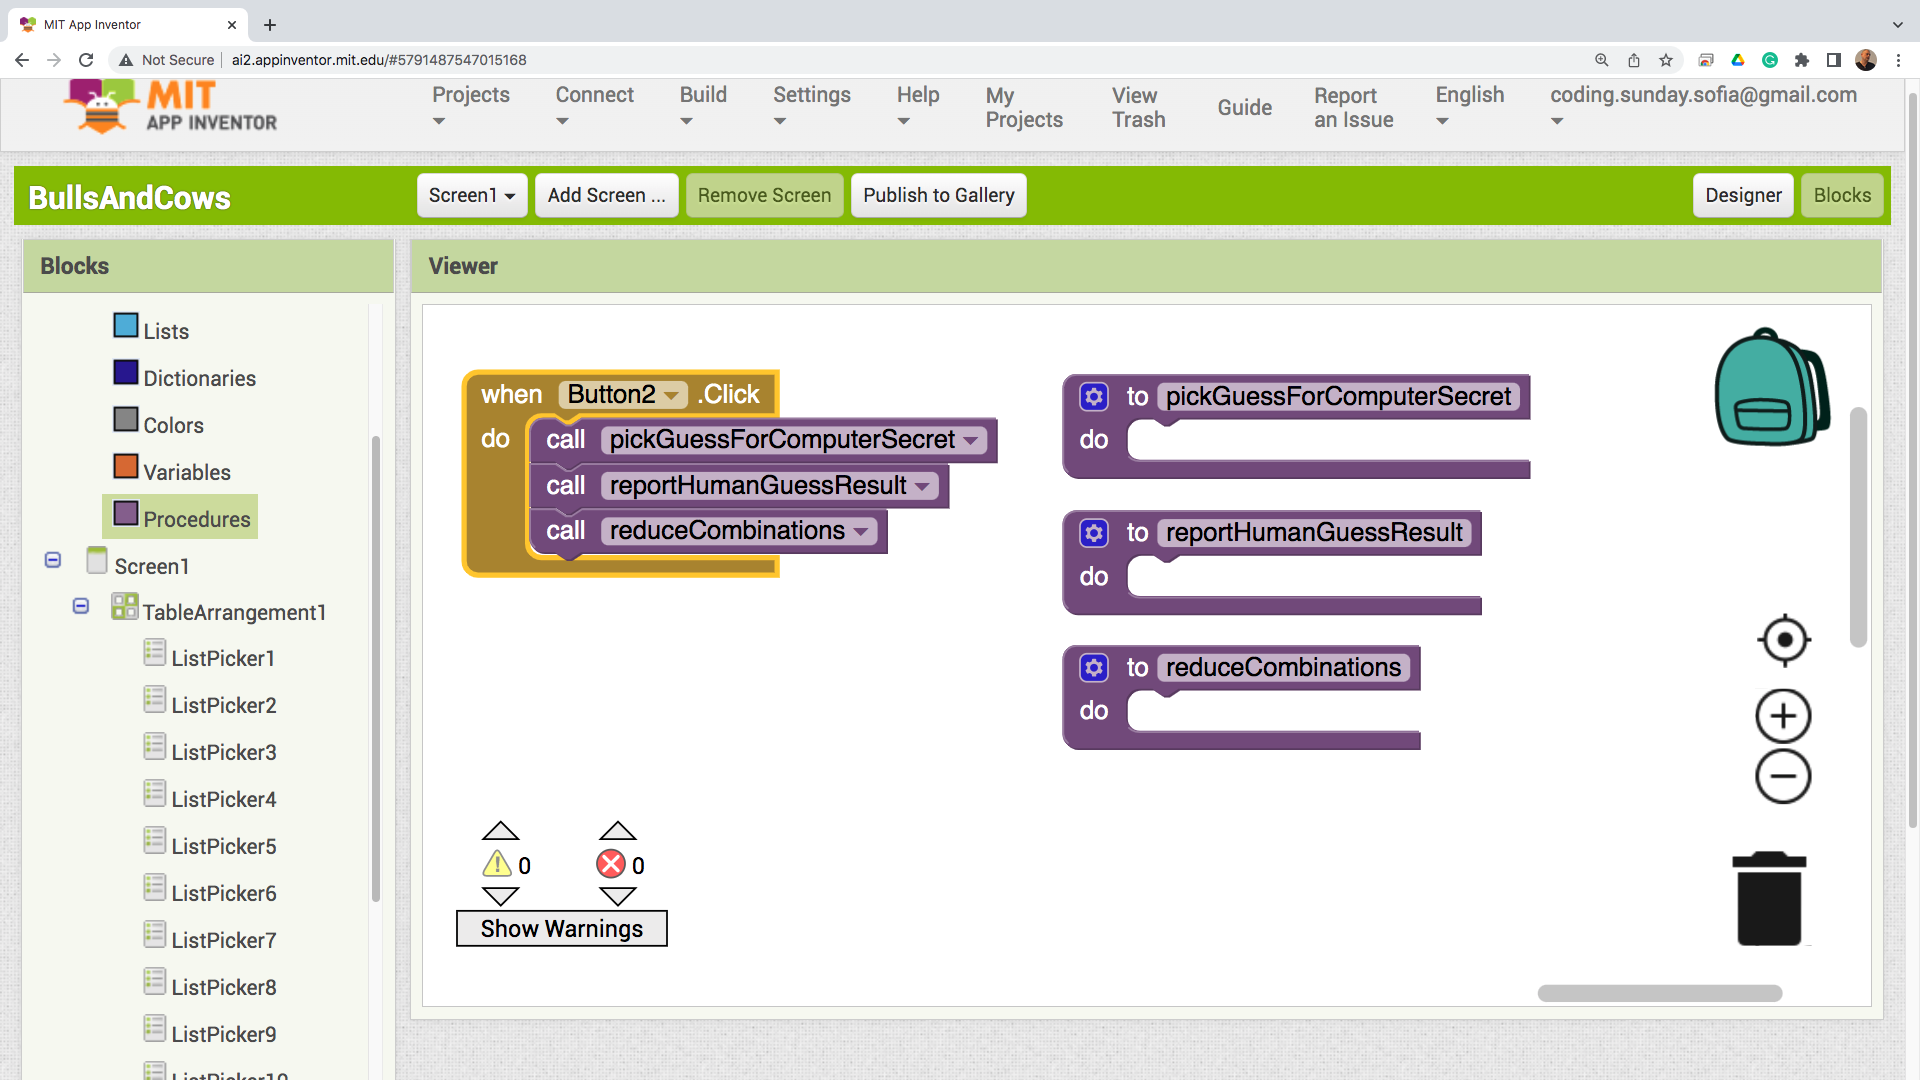
\includegraphics[width=1.0\linewidth,height=0.5\linewidth]{fig080018.png}
   \caption{First Button Actions}
\label{fig080018}
\end{figure}

The human's guess is taken from the visual controls, and each digit is lumped together and written to the auxiliary global variable (Fig. \ref{fig080019}).

\begin{figure}[H]
   \centering
   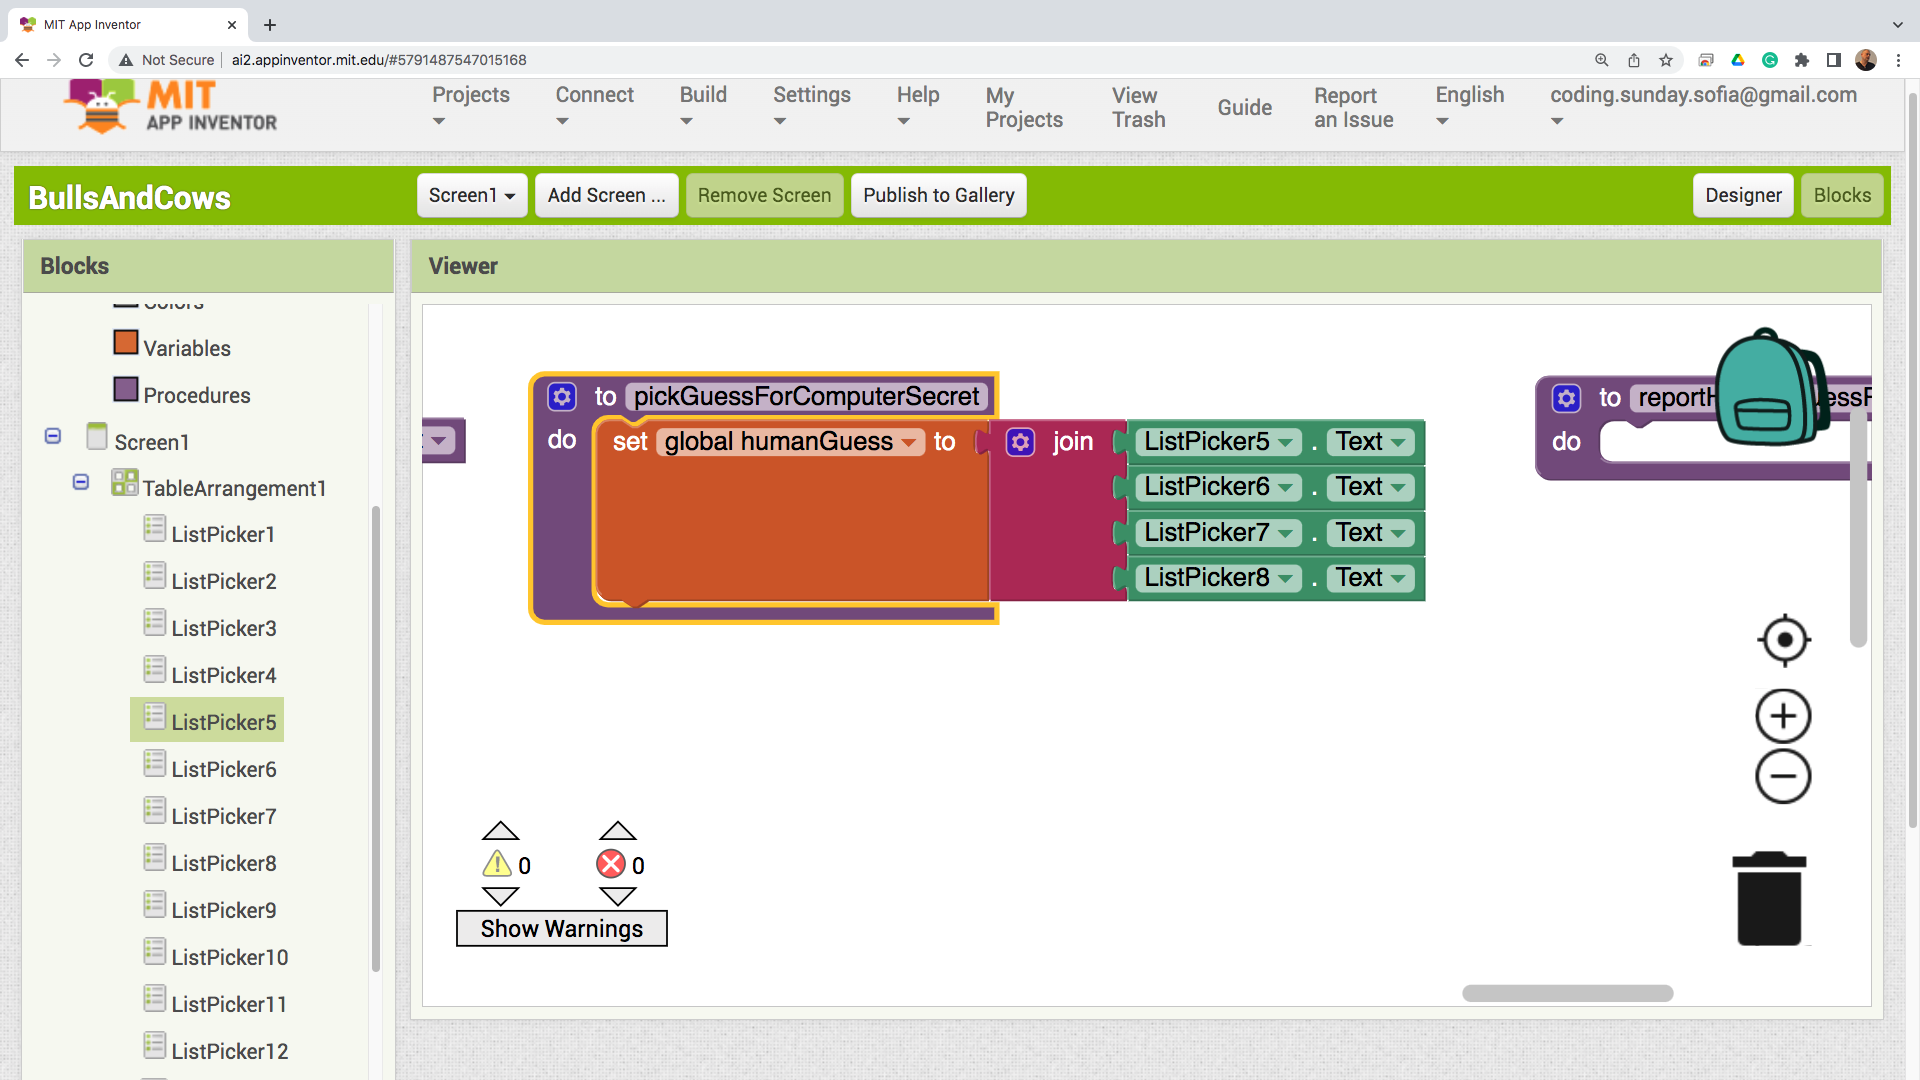
\includegraphics[width=1.0\linewidth,height=0.5\linewidth]{fig080019.png}
   \caption{Taking the guesswork out of the human}
\label{fig080019}
\end{figure}

The number of bulls and cows known by the human is determined by a helper procedure that returns a list of two elements. The first element contains the number of bulls and the second element the number of cows. To calculate these numbers, the computer opponent's secret number and the guess made by the player are used (Fig. \ref{fig080020}). The result is displayed in the last two components of the GUI.

\begin{figure}[H]
   \centering
   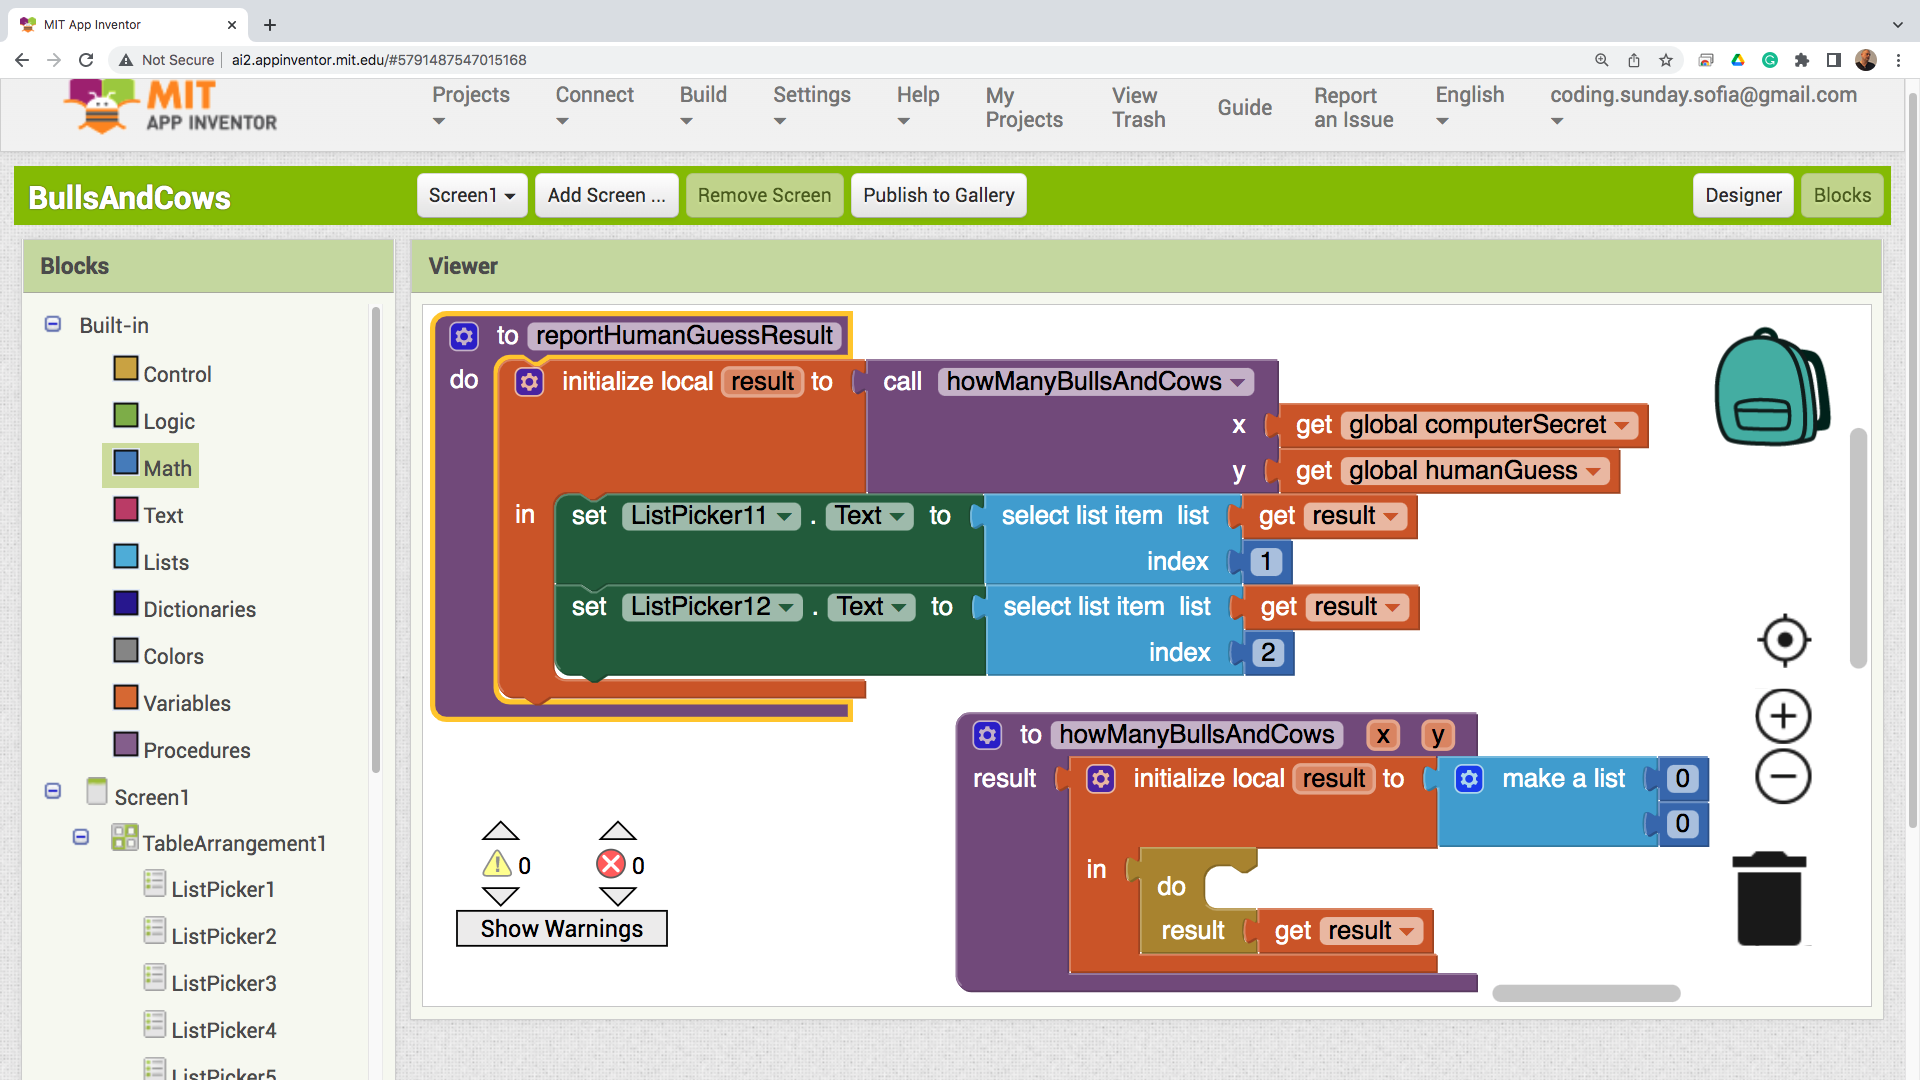
\includegraphics[width=1.0\linewidth,height=0.5\linewidth]{fig080020.png}
   \caption{Visualization of the number of bulls and cows known to man}
\label{fig080020}
\end{figure}

To reduce the number of combinations, the result of checking the assumption made, that is, the number of bulls and cows reported by the person, should be taken. This is accomplished with a helper procedure that also returns a list whose first element contains the number of bulls and the second element the number of cows (Fig. \ref{fig080021}).

\begin{figure}[H]
   \centering
   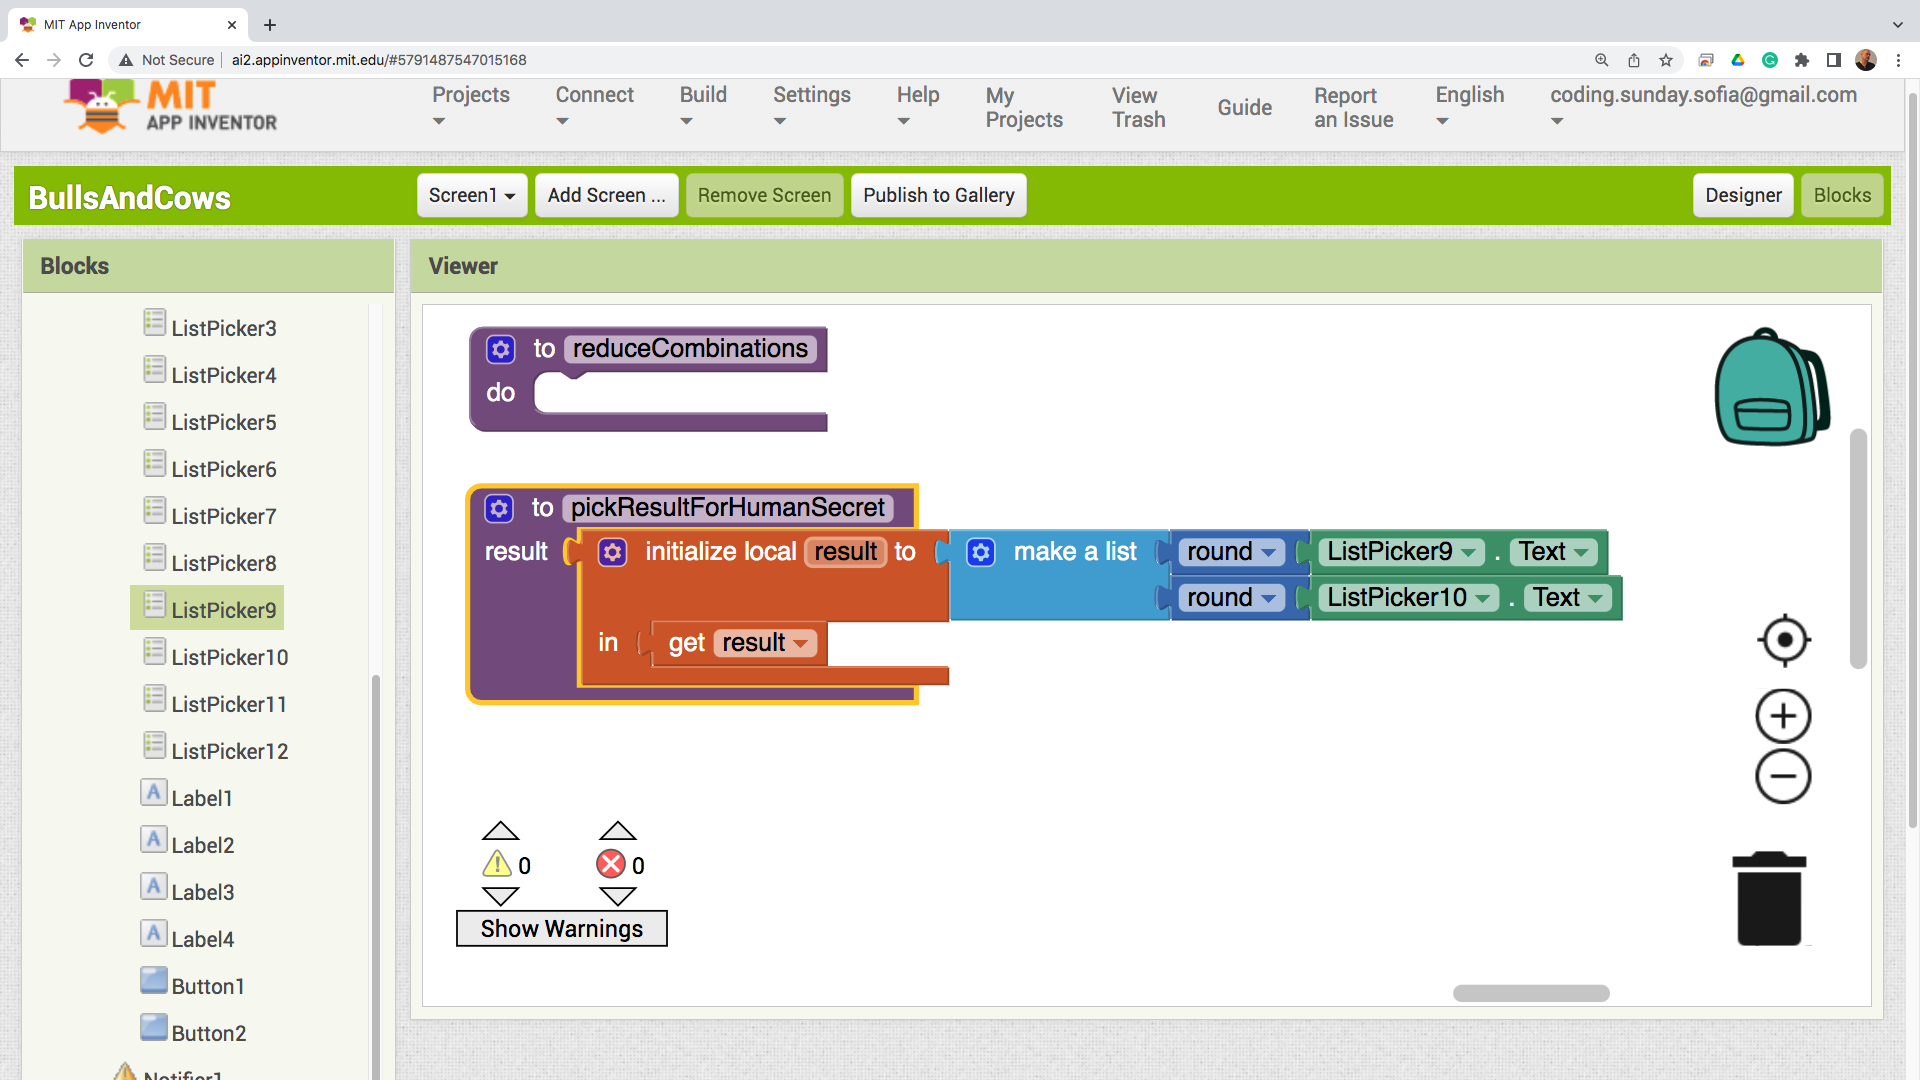
\includegraphics[width=1.0\linewidth,height=0.5\linewidth]{fig080021.png}
   \caption{Retrieving the number of bulls and cows declared by the person}
\label{fig080021}
\end{figure}

Weeding out unnecessary combinations is done by taking the answer given by the human opponent. After that, a new empty list is created, in which only the numbers that meet the criteria specified in the response will enter the list. Screening is achieved by traversing the list of combinations (Fig. \ref{fig080022}). Each combination is fed to the utility function to determine how many bulls and cows the combination makes, based on the guess made by the computer opponent. If the currently checked combination has the same characteristics (number of bulls and number of cows) as the characteristics returned by the human opponent, then the current combination enters the new list. After traversing the list of combinations completely, the old list is replaced with the new list.

\begin{figure}[H]
   \centering
   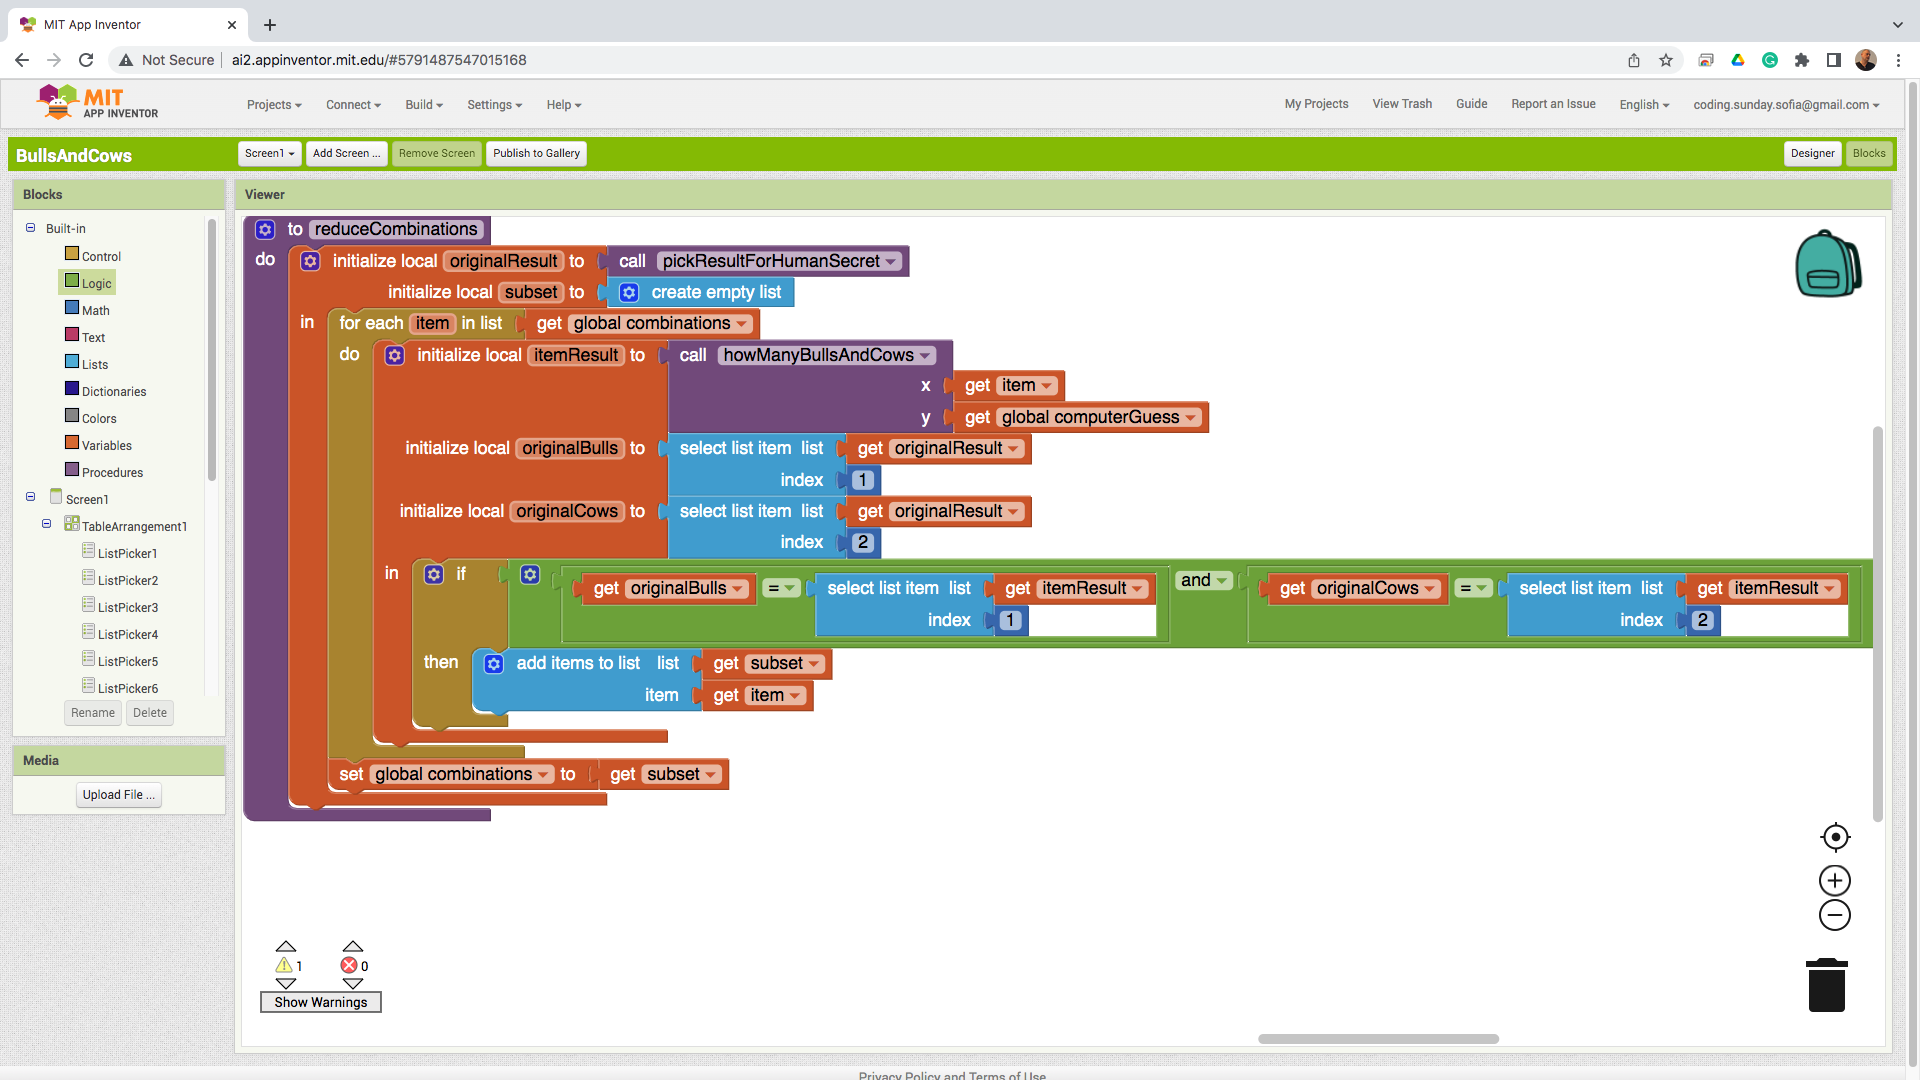
\includegraphics[width=1.0\linewidth,height=0.5\linewidth]{fig080022.png}
   \caption{Weeding out unnecessary combinations}
\label{fig080022}
\end{figure}

The calculation of the number of bulls and the number of cows for two numbers is done by rotating two loops. One cycle traverses the first number, digit by digit, and the second cycle the second number, again digit by digit (Fig. \ref{fig080023}).

\begin{figure}[H]
   \centering
   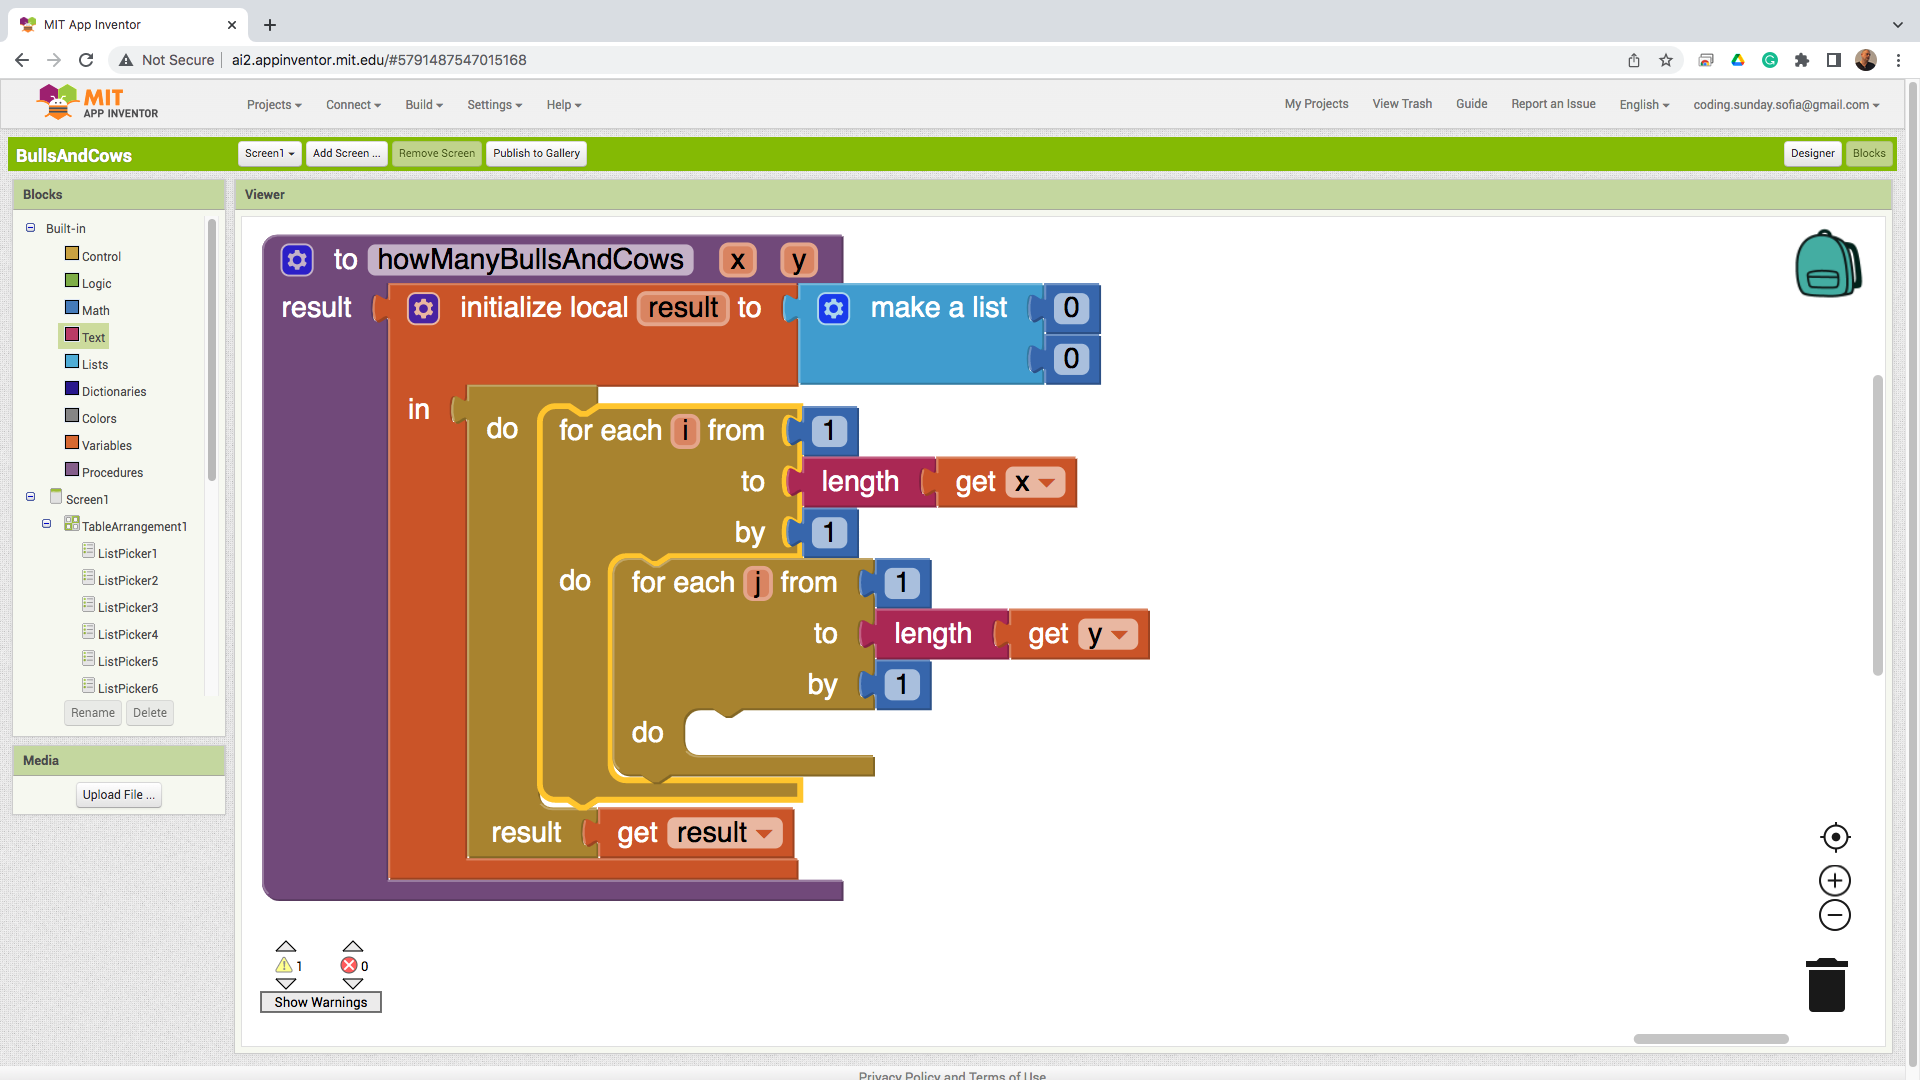
\includegraphics[width=1.0\linewidth,height=0.5\linewidth]{fig080023.png}
   \caption{Treading the digits of two numbers}
\label{fig080023}
\end{figure}

The currently viewed digits of the two numbers are loaded into two auxiliary variables (Fig. \ref{fig080024}). With these two variables and with the cycle counters, the necessary comparisons are made for the presence of a bull or a cow.

\begin{figure}[H]
   \centering
   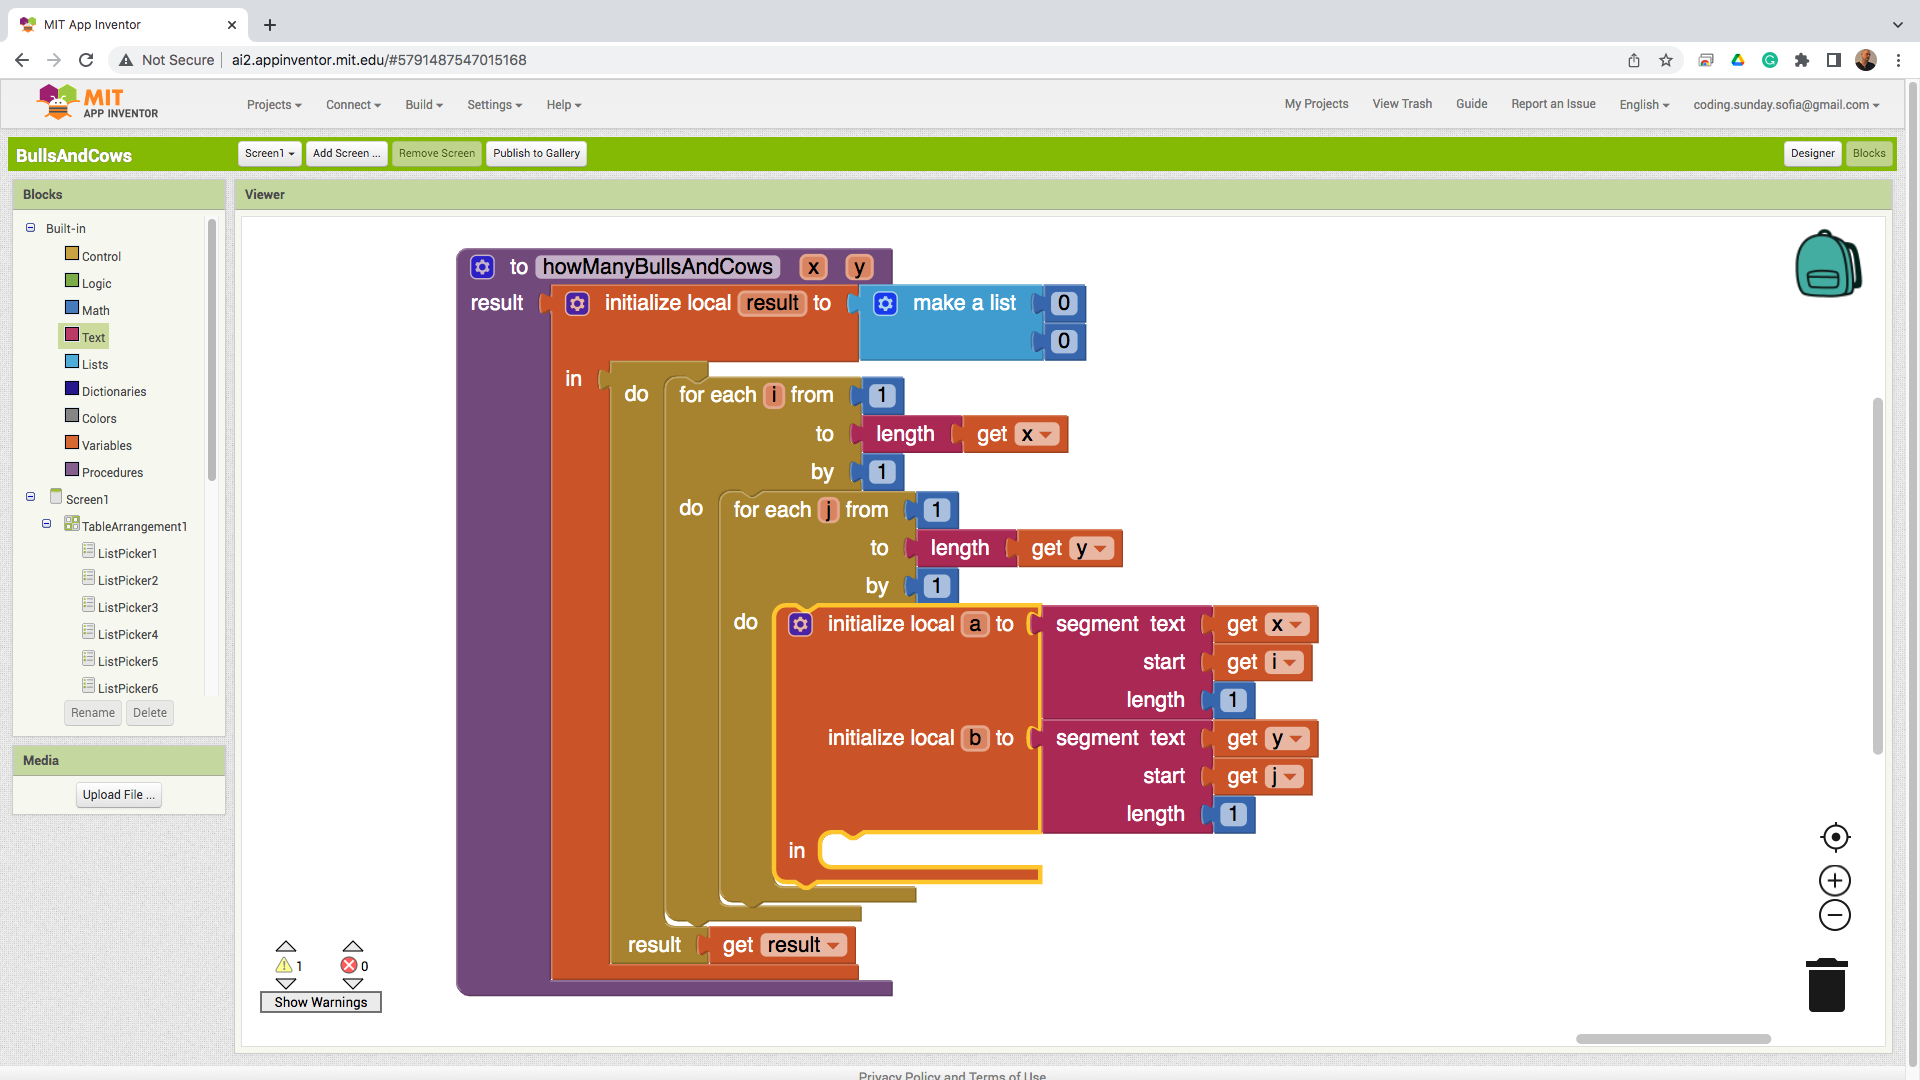
\includegraphics[width=1.0\linewidth,height=0.5\linewidth]{fig080024.png}
   \caption{Helper variables for the numbers}
\label{fig080024}
\end{figure}

If the two numbers match, it means either a bull or a cow (Fig. \ref{fig080025}). Whether the match is a bull or a cow is determined by the values of the counters for the two cycles.

\begin{figure}[H]
   \centering
   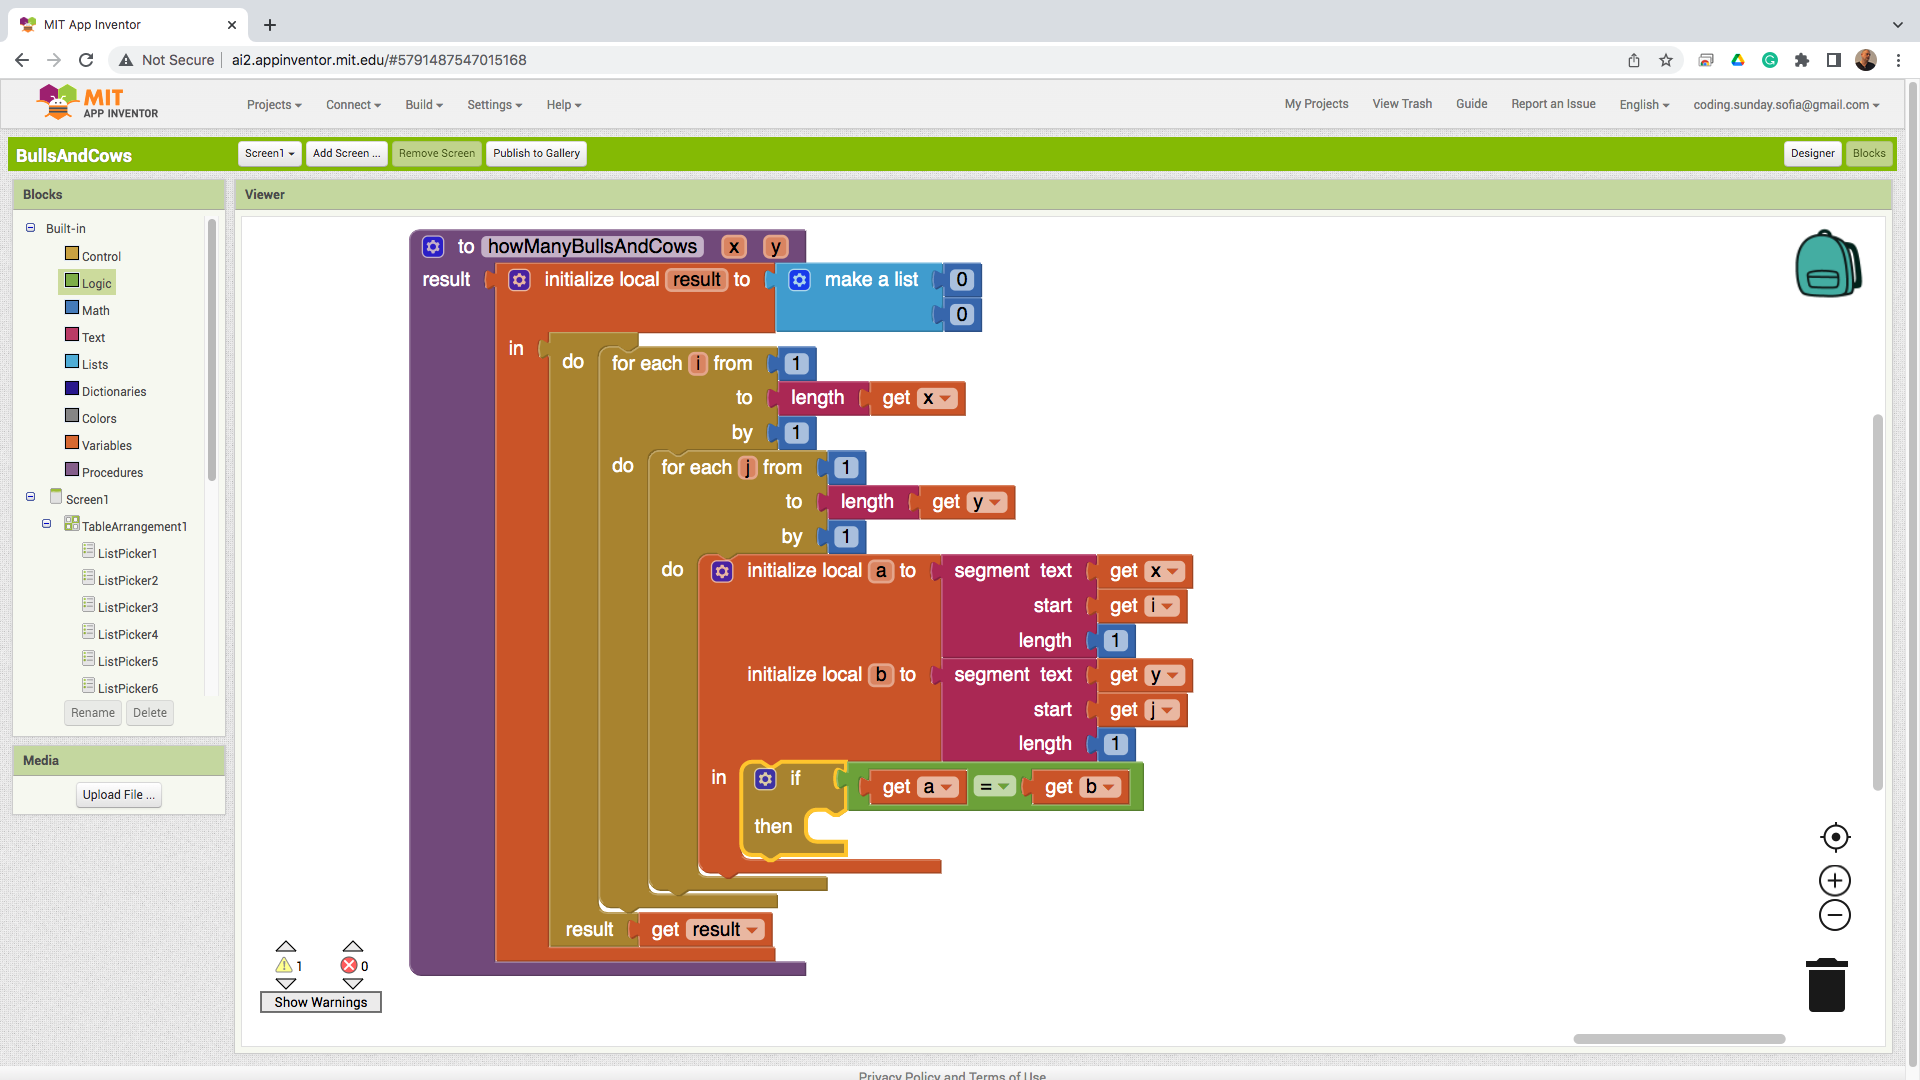
\includegraphics[width=1.0\linewidth,height=0.5\linewidth]{fig080025.png}
   \caption{Number Match}
\label{fig080025}
\end{figure}

If the two counters have the same value, then a bull is present, otherwise it is a cow (Fig. \ref{fig080026}).

\begin{figure}[H]
   \centering
   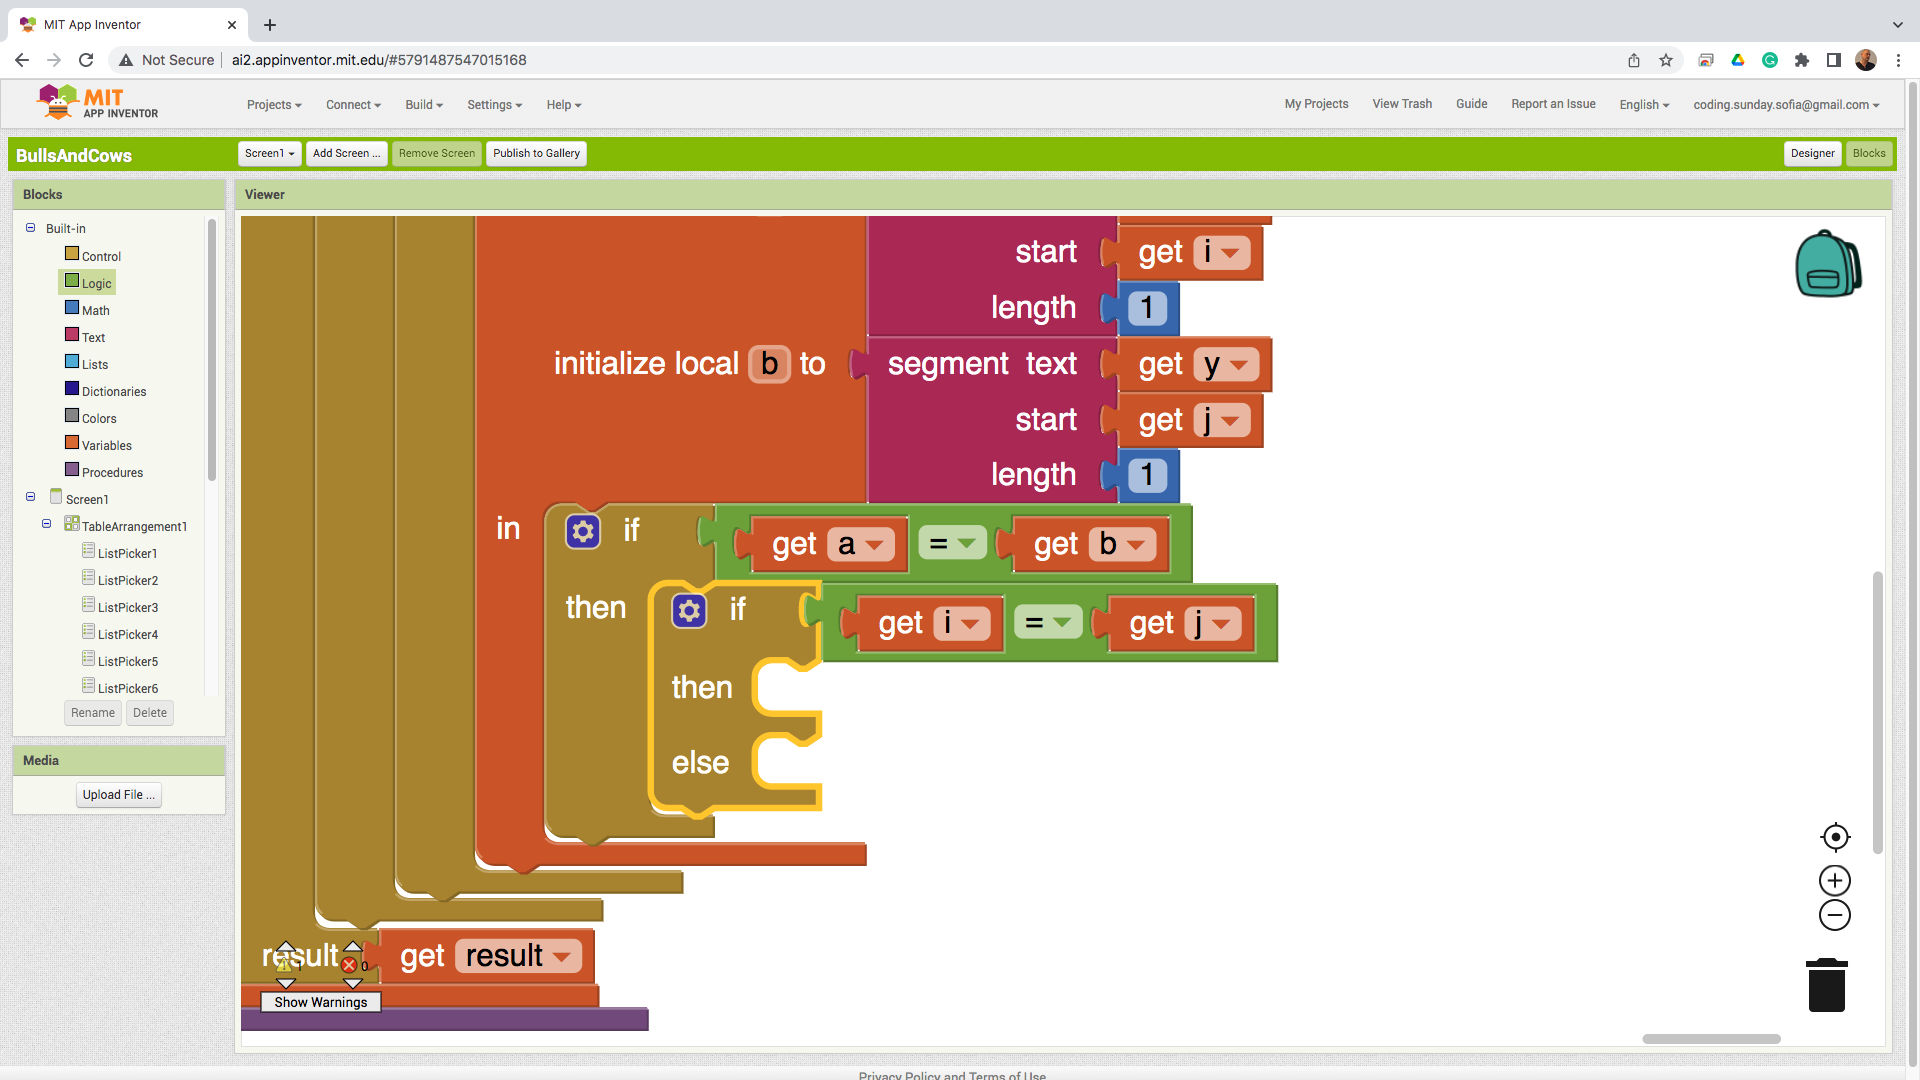
\includegraphics[width=1.0\linewidth,height=0.5\linewidth]{fig080026.png}
   \caption{Counter match}
\label{fig080026}
\end{figure}

Encountering a bull increases the value of the first element in the result by one, and encountering a cow increases the value of the second element of the result list by one (Fig. \ref{fig080027}).

\begin{figure}[H]
   \centering
   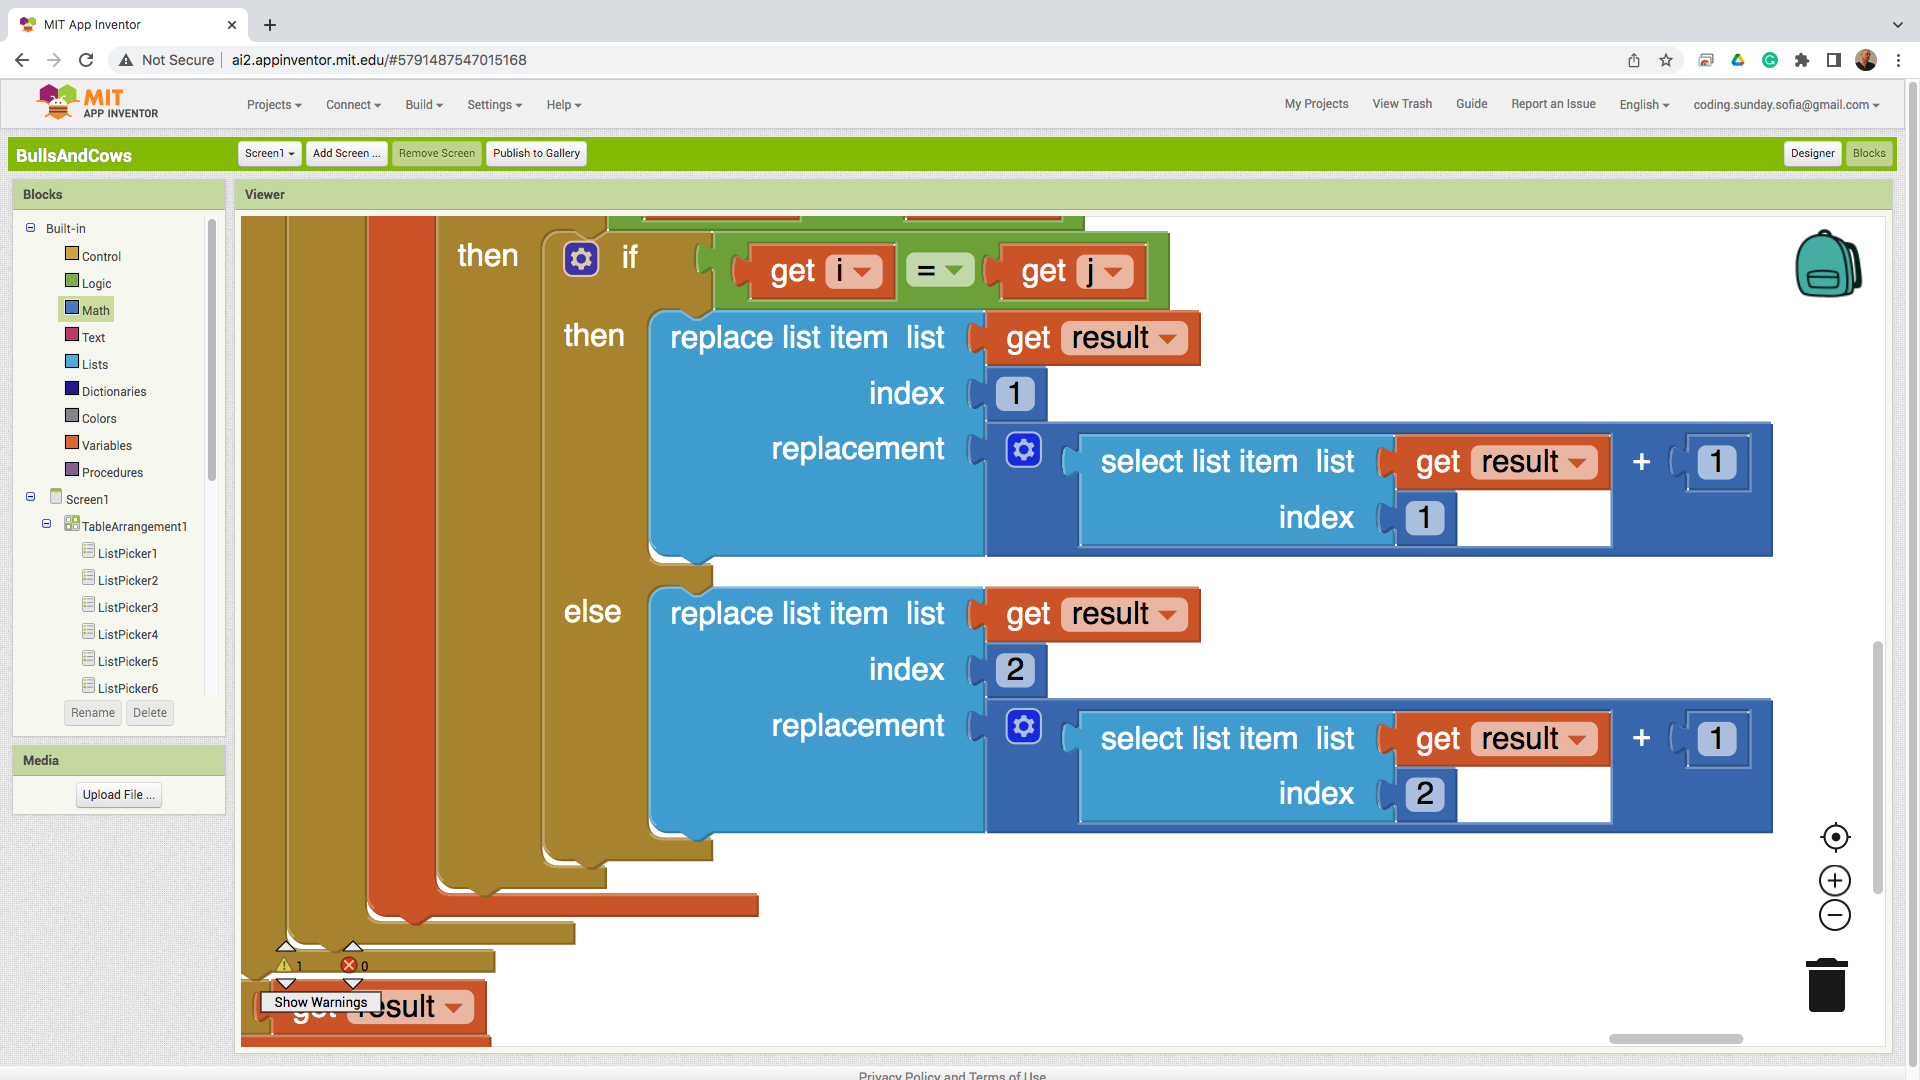
\includegraphics[width=1.0\linewidth,height=0.5\linewidth]{fig080027.png}
   \caption{Counting the bulls and cows}
\label{fig080027}
\end{figure}

The game is played in sequence (Fig. \ref{fig080028}) by pressing the first button first. Pressing the first button allows the computer opponent to guess the human opponent's secret number. Then, the human marks how many bulls and how many cows the computer opponent was able to guess. The third step is for the human opponent to make their guess about the computer opponent's secret number. The second button is pressed, in which the computer opponent reports how many bulls and how many cows the human guessed.

\begin{figure}[H]
   \centering
   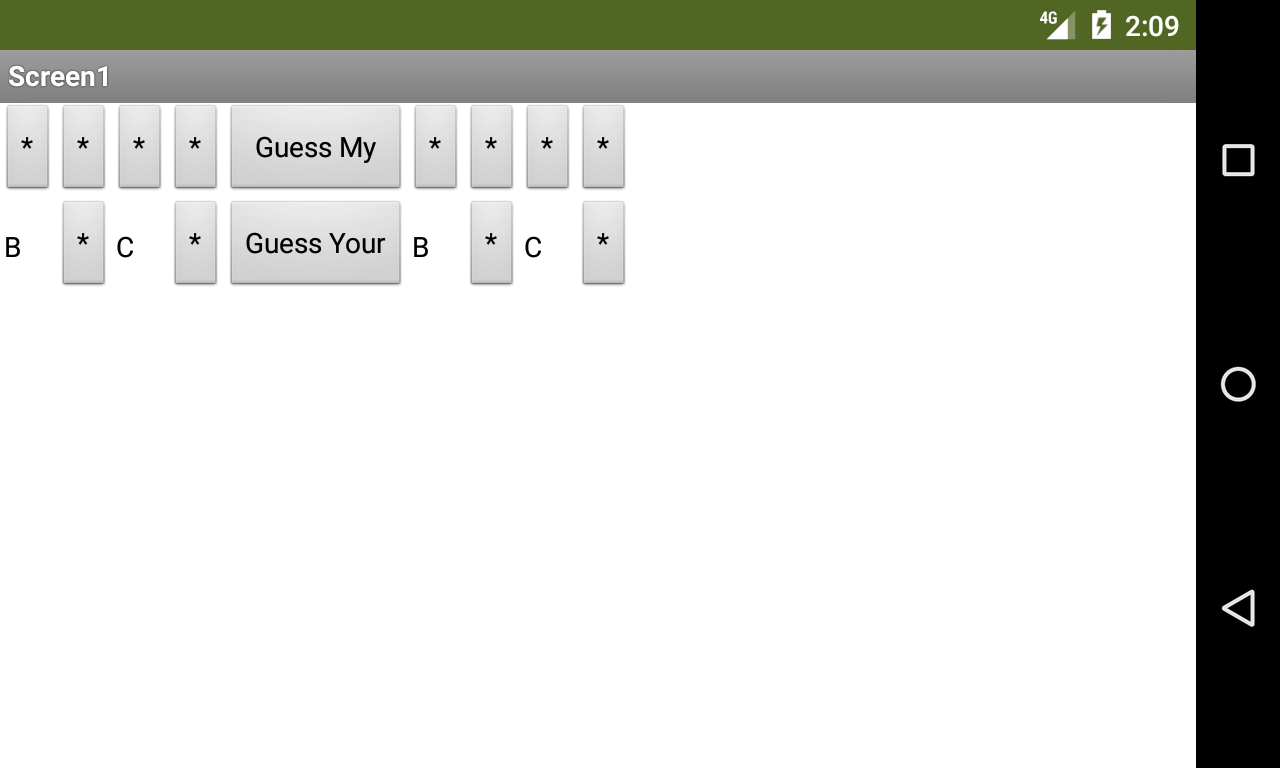
\includegraphics[width=1.0\linewidth,height=0.5\linewidth]{fig080028.png}
   \caption{Game Home Screen}
\label{fig080028}
\end{figure}

By following the sequence of steps for working with the graphical interface (Fig. \ref{fig080029}), the game continues until one of the players hits four bulls.

\begin{figure}[H]
   \centering
   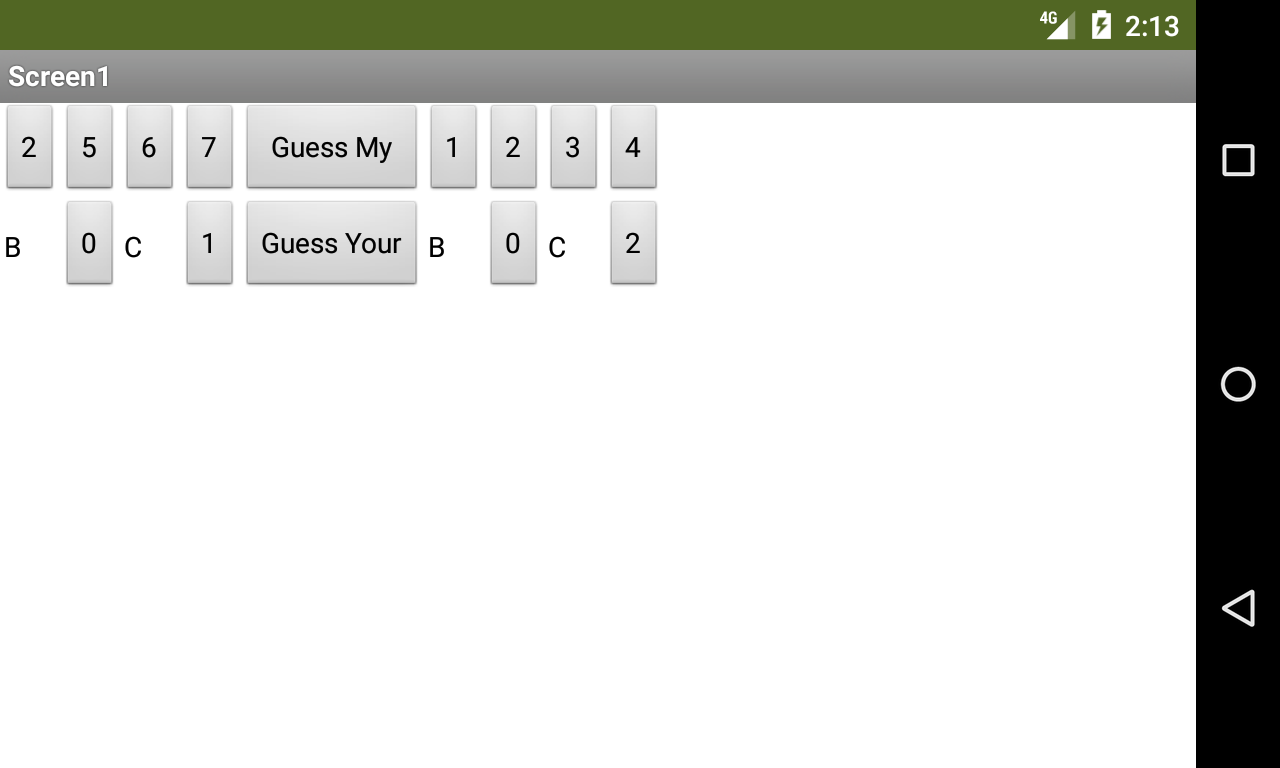
\includegraphics[width=1.0\linewidth,height=0.5\linewidth]{fig080029.png}
   \caption{Intermediate game move}
\label{fig080029}
\end{figure}

\section{Publish the project}

After reaching a fully functional version of the game, the project can be published in the gallery so that it is available to a wide audience (Fig. \ref{fig080030}).

\begin{figure}[H]
   \centering
   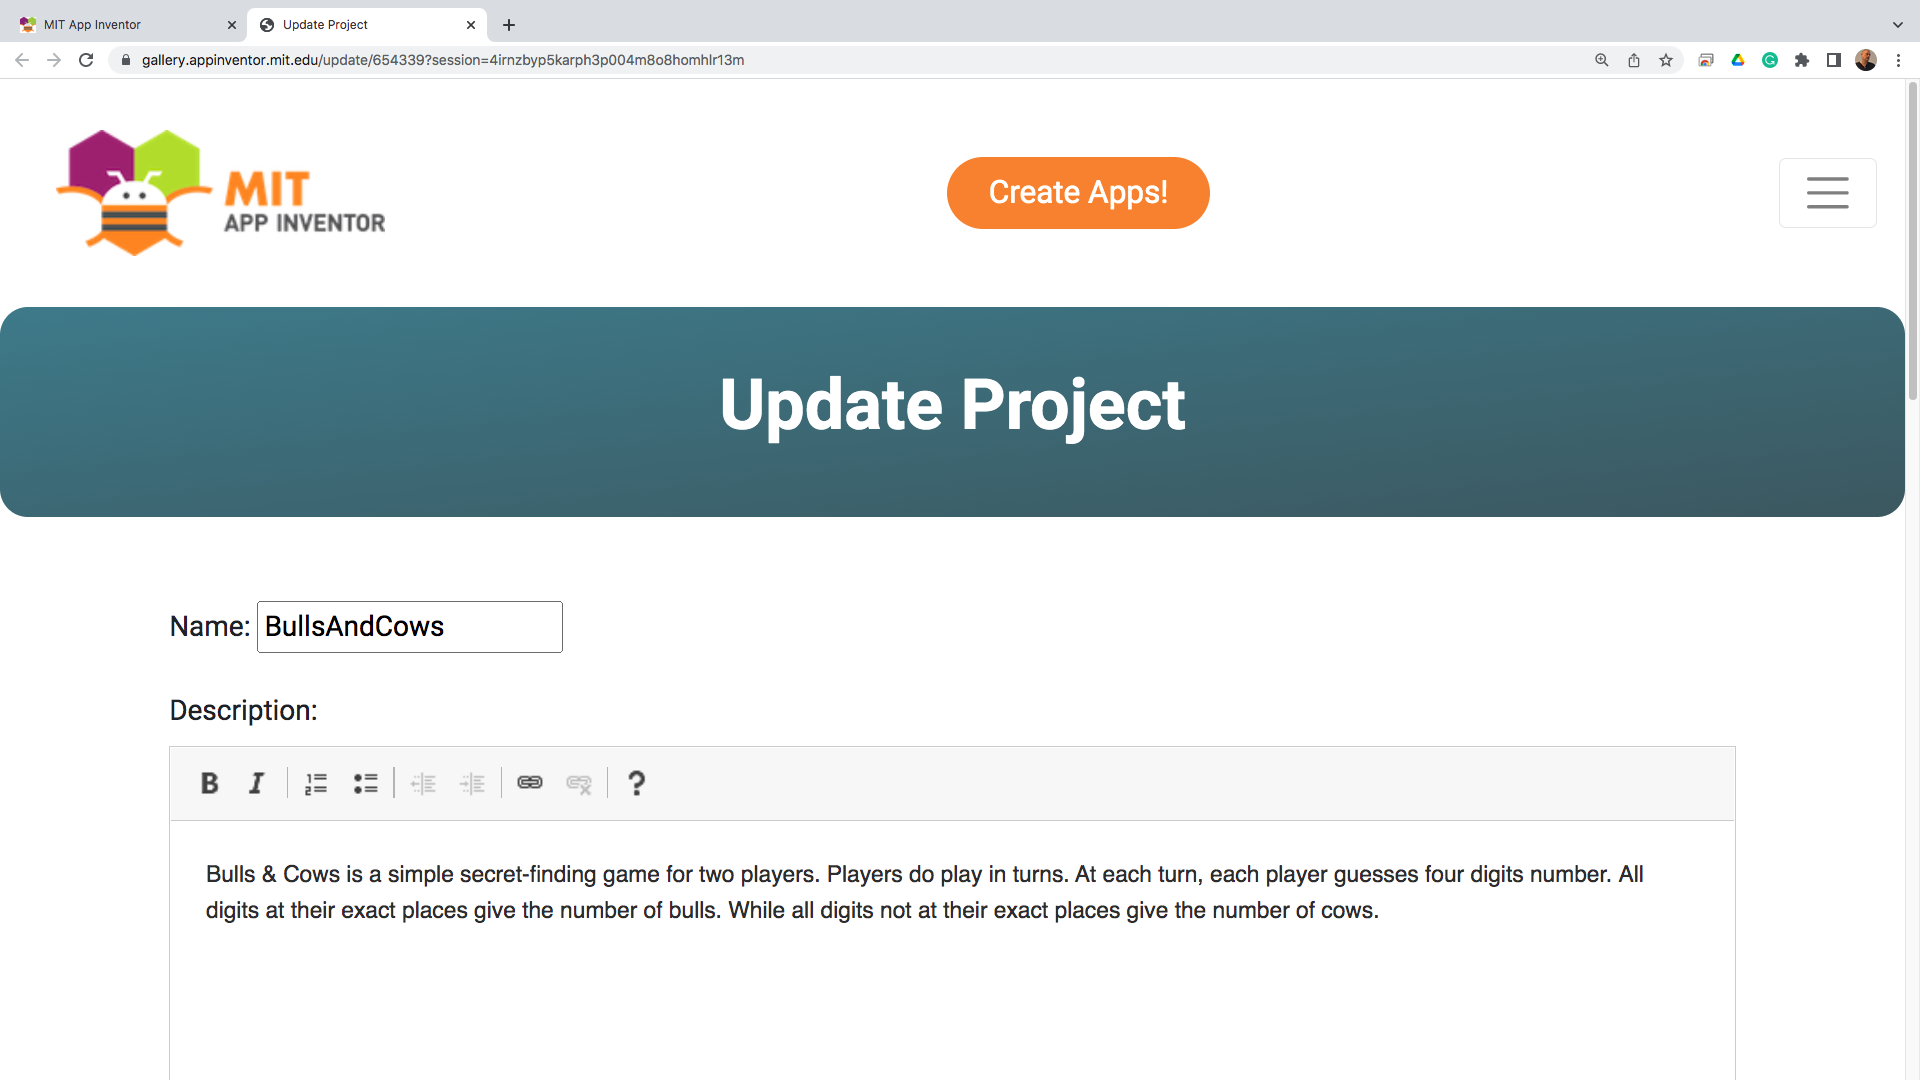
\includegraphics[width=1.0\linewidth,height=0.5\linewidth]{fig080030.png}
   \caption{Project Description}
\label{fig080030}
\end{figure}

After publishing, hyperlinks appear on the application page to run the program or view its code in the development environment (Fig. \ref{fig080031}).

\begin{figure}[H]
   \centering
   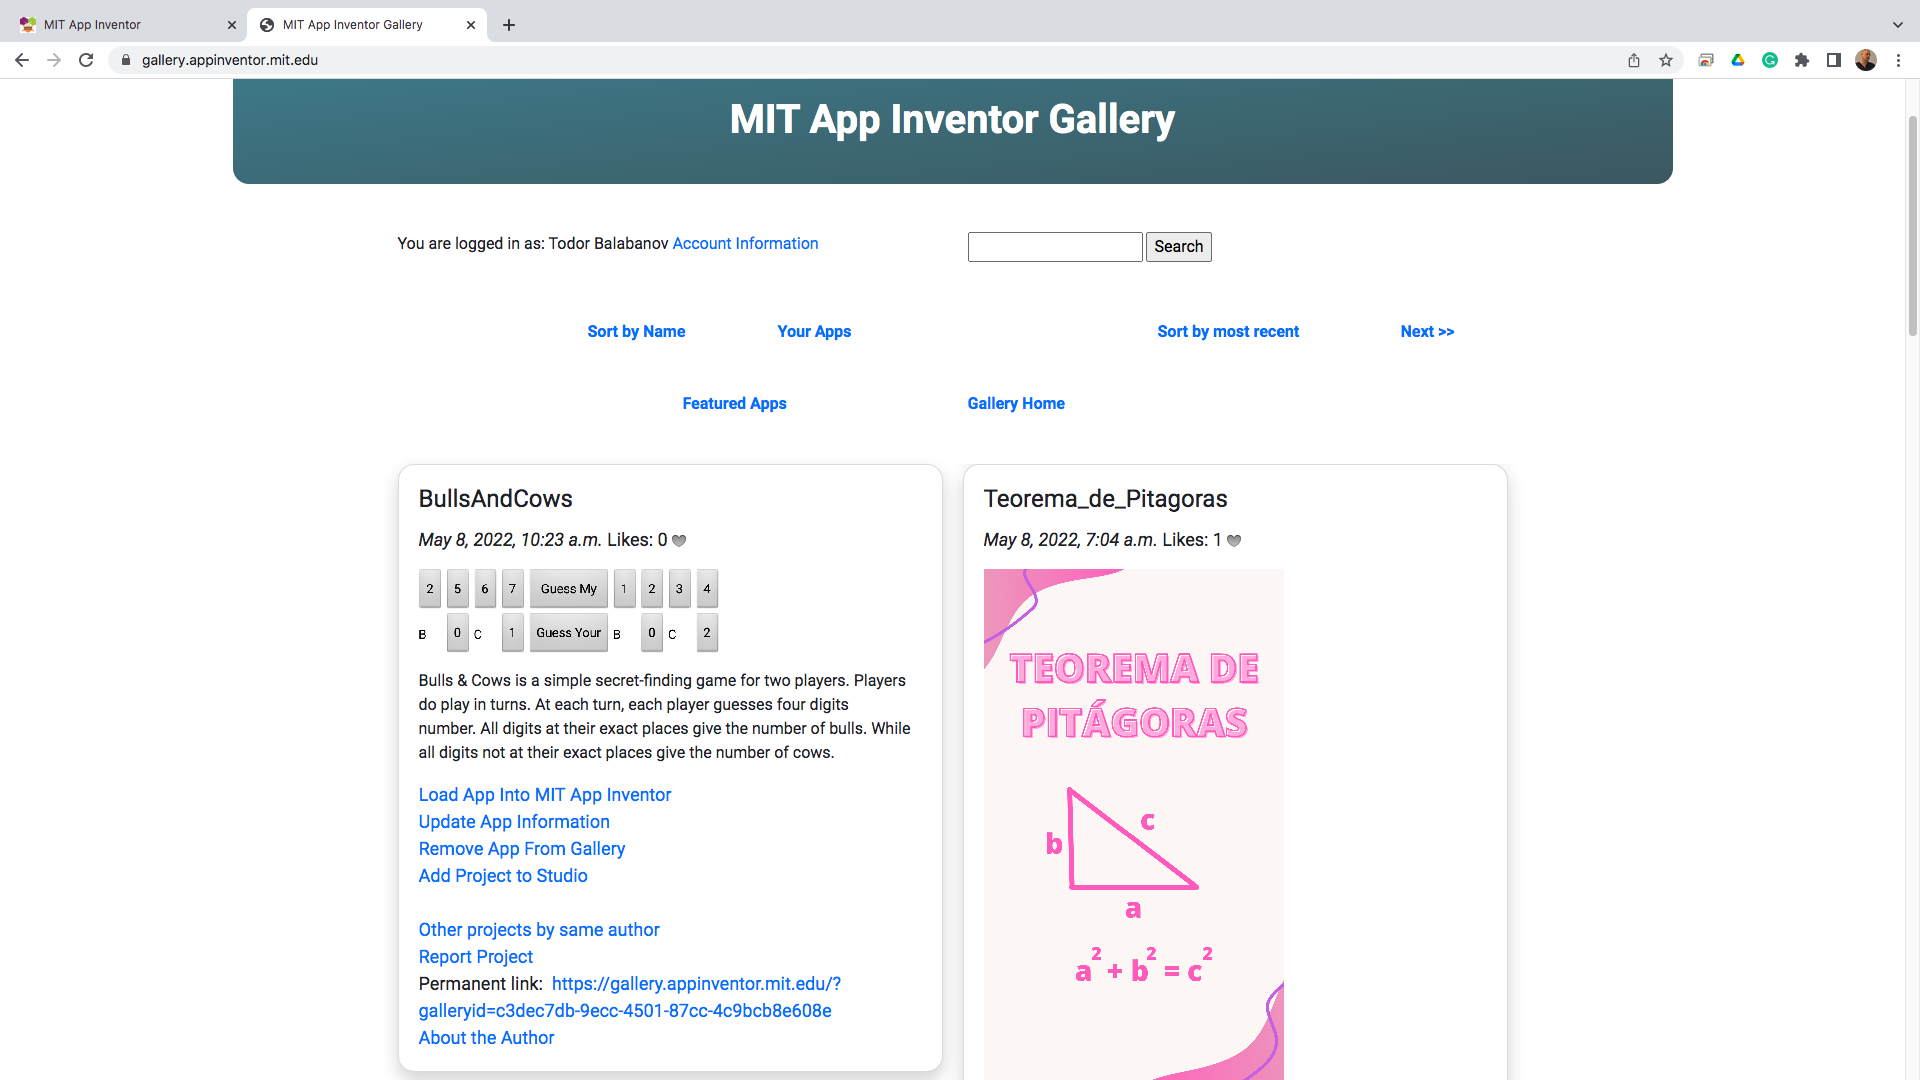
\includegraphics[width=1.0\linewidth,height=0.5\linewidth]{fig080031.png}
   \caption{Published Project Page}
\label{fig080031}
\end{figure}

Although fully functional, the game is still not finished to the level of a final product. A series of checks to ensure that the user is entering numbers correctly (eg repeating digits) are missing. There is no functionality to announce the winner, although the appearance of four bulls clearly indicates who wins. It lacks a help screen as well as a sound layout. The missing functionality is beyond the scope of this presentation and could serve as an additional exercise for those wishing to upgrade their knowledge.
